\documentclass[11pt,a4paper,twoside,twocolumn]{article}

\usepackage{graphicx,parskip,times,amsfonts,amsmath}
%\usepackage{url}
%\usepackage{html}
\usepackage{esc-handbook-org}
\usepackage{eurosym}
%\usepackage{chapterbib}
\usepackage{apalike}
\usepackage{a4,a4wide}
\usepackage[english]{babel}
\usepackage{amssymb,amsmath,amsfonts}
\usepackage{bibunits}

%---------------------PDF-definitions--------------------------------------
\usepackage[pdftex,           %%% hyper-references for pdflatex
  hypertexnames=false,%       %%% needed for correct links to figures
  breaklinks=true,%           %%% break links if exceeding a single line
  colorlinks=true,
  linkcolor=black,%           %%% to underline links instead of boxing
  urlcolor=blue]{hyperref}    %%% blue instead of cyan URLS
%---------------------end-of-PDF-definitions-------------------------------


\newcommand{\mycaption}[1]{\caption{{\footnotesize #1}}}
\renewcommand*{\cleardoublepage}{\clearpage\if@twoside \ifodd\c@page\else
    \hbox{}
    \if!\blankpagetext!\else
    \vfil \begin{center} \setlength{\fboxsep}{3mm}%
    \framebox{\blankpagetext}
    \end{center}\vfil\vfil \fi
    \newpage\if@twocolumn\hbox{}\newpage\fi\fi\fi}
\newcommand*{\resetpages}{\cleardoublepage\pagenumbering{arabic}}
\raggedbottom \pagenumbering{Roman}

\setlength{\parskip}{1ex plus 1ex}

\begin{document}
% Robert's hack:
\renewcommand{\refname}{Publications}
\renewcommand{\bibname}{Publications}

\def\Hchapter{\paragraph}
%
\title     {Jacobs Center \\
            Research Report 2006} \shorttitle{JCLL RP 2006}
\author    {Anke Allner}
\date      {December 2006}
\masterfile{JCLL--RR--2006} \issue     {0} \revision {1} \version
{2}{0}{27.12.06}{Test}

\hyphenation{know-ledge stra-te-gy}

\onecolumn
\shorttitle{Table of Contents} \tableofcontents \resetpages  
\twocolumn
\input{intro}
\cleardoublepage
\hyphenation{Life-long}
\section{The Neuroscience and Human-Performance Perspective on
Lifelong Learning} \shorttitle{Neuroscience and Human Performance
}

  Our research focuses on identifying mechanisms underlying cortical plasticity and the structure-function relationships between cognitive, sensory, and motor performance and learning. The human brain remains plastic even at high age. However, plastic capacity declines with age. In this context the ability to facilitate plasticity is of high significance for the elder learner.
  
 In this context, research of our group is divided into three main topics:

 Our first interest is to investigate the plastic-adaptive capacity of the brain to understand basic mechanisms of plasticity and learning as well as the effects of age. Based on these experiments possible interventions might be developed to improve learning and to interfere with age-related decline. Fields of research are vibrotactile perceptual learning, force control and force modulation, motor-cognitive dual-task performance, intermanual transfer of learned motor programs, and the sensory-motor coupling during learning.
	
 Second, physical fitness is assumed to preserve cognitive functioning and psychological well-being in older adults. However, the mechanisms, the dose-response-relationship and also effects of different types of exercise are not well understood. Following an interdisciplinary view on human performance that comprises motor, neurophysiological, and psychological expertise and methods, the second area of research deals with the role of aerobic and acrobatic exercise on cognitive performance and well-being across the lifespan.
	
 Third, the plastic-adaptive capacities of the adult and aging brain are of particular importance for the aging work force. As part of joint JCLL efforts, combining our expertise in the above mentioned fields of research, we developed a research proposal to establish measures of older workers' adaptivity in the sensory, motor and cognitive domains and to relate their adaptive capabilities to the demands of the work place. From the results we will be able to identify mismatches between demands of the work place and individual preconditions. We assume that these mismatches might be used as predictors of low productivity or health problems of the employees.

\subsection{Plastic-Adaptive Capacity of the Brain: Mechanisms, Effects of Age, Possible Interventions}


\index{Godde, Ben}

\paragraph{Research Team}
Ben Godde (Professor), Claudia Voelcker-Rehage (Postdoctoral Fellow), Mikhail Babanin (Doctoral Fellow), Alexander Knop (Diploma Student, University of Bremen).

First, within the sensory domain we are interested in the plastic-adaptive competencies related to tactile processing of younger and older adults. Using functional MRI and psychophysics we investigate the cortical topography of tactile perception and the cortical mechanisms of perceptual learning.
	
	Second, within the motor domain, we are mainly interested in upper extremity force control. Control of the fine finger forces is an elementary component of movement production of many daily activities (e.g. dressing, eating, opening containers) and its assessment provides insight into movement control and coordination. A decline in force control is common in older adults. We examine age-related differences in force control, practice effect on force modulation, and age-related differences in dual-task performance. Besides force control we are interested in the intermanual transfer of learned motor programs.
	
	In a third line of research we are going to focus on the interaction between motor and sensory performance. Particularly, we are interested in the following questions: (1) Does high frequency tactile stimulation help to diminish age-related performance decrements in force control? 
	
\newpage
(2) Does high frequency tactile stimulation facilitate sensory and/or motor learning? These questions are the first steps in developing appropriate interventions to improve manual dexterity in older adults.

\null
\textbf{Research Highlights 2006}


\textit{Effects of high frequency tactile stimulation on sensory and motor performance in younger and older adults}

	It is assumed that an important mechanism responsible for precise force control is tactile sensitivity. However, also contradictory results exist and the neural control mechanisms responsible for precise manipulation of grasping forces are largely unknown. We examined the link between motor and tactile domains by applying an intervention paradigm of high frequency ($\sim$20Hz) tactile stimulation (tHFS). This protocol is assumed to induce long-term potentiation (LTP) like effects in the neocortex and has recently been shown to profoundly improve tactile acuity. 

	Younger (18-28 years of age) and older (65-75 years of age) right handed participants were randomly assigned to an experimental and a control group. Before and after 30 minutes of tHFS on the index finger and thumb of the left hand, participants performed different tactile (spatial and temporal discrimination) and motor tasks (unimanual isometric precision grip task using a Mini Model force transducer and Purdue Pegboard test) with their stimulated fingers.
	
	Results indicated that tHFS significantly improved tactile frequency discrimination of the left index finger, whereas motor performance as assessed with the pegboard task was impaired (see Figure \ref{fig:profBenGodde}). These effects were found for both age groups with similar effect sizes even though absolute levels of performance in all tasks were lower for older as compared to younger adults. For the precision grip task younger subjects of both the experimental and control group similarly improved from the pre to the post test. Contrary, only older subjects which received the tHFS intervention could profit from the test repetition whereas the performance of the older control group remained stable. 
	
	Our results suggest that reorganization of the somatosensory cortex presumably induced by the applied protocol of passive tactile stimulation not only promotes sensory performance but also significantly affects fine motor control of the respective fingers. Moreover, our study reveals the remaining plastic capacity of the older brain (Voelcker-Rehage, Knop, Babanin \& Godde, 2006). 

%\begin{figure}[ht]
%  \begin{center}
%    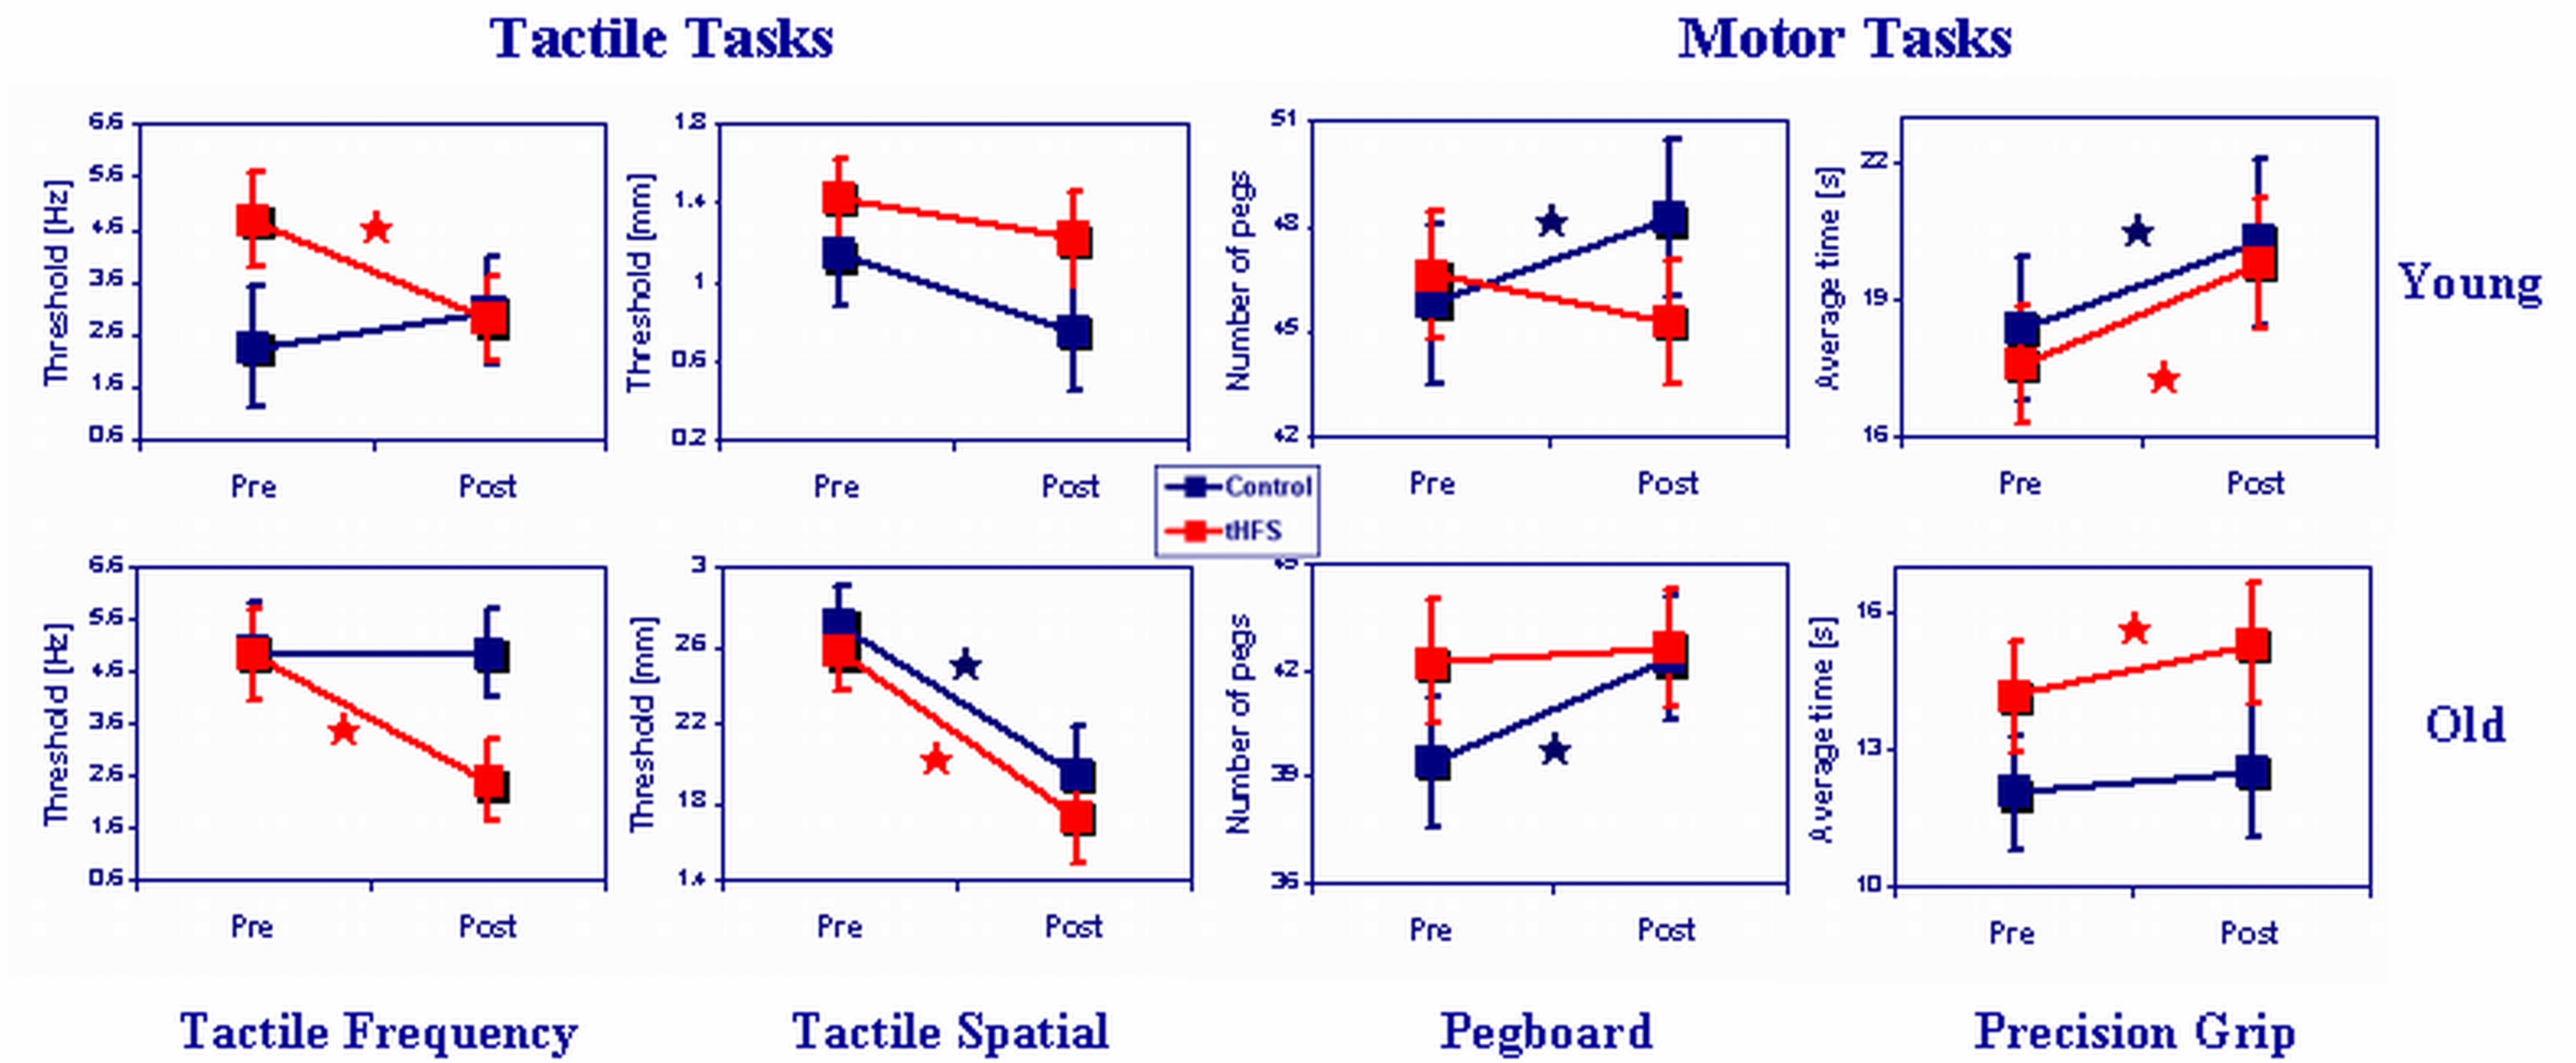
\includegraphics[width=7.5cm]{profBenGodde-fig1.jpg}
%    \caption{Differential effects of tHFS on tactile (left 2 columns) and motor (right 2 columns) performance in young %(top) and old (bottom) subjects. Experimental group shown in red, control group in blue.}\label{fig:profBenGodde}
%   \end{center}
%\end{figure}

\begin{figure}[htb]
  \begin{center}
    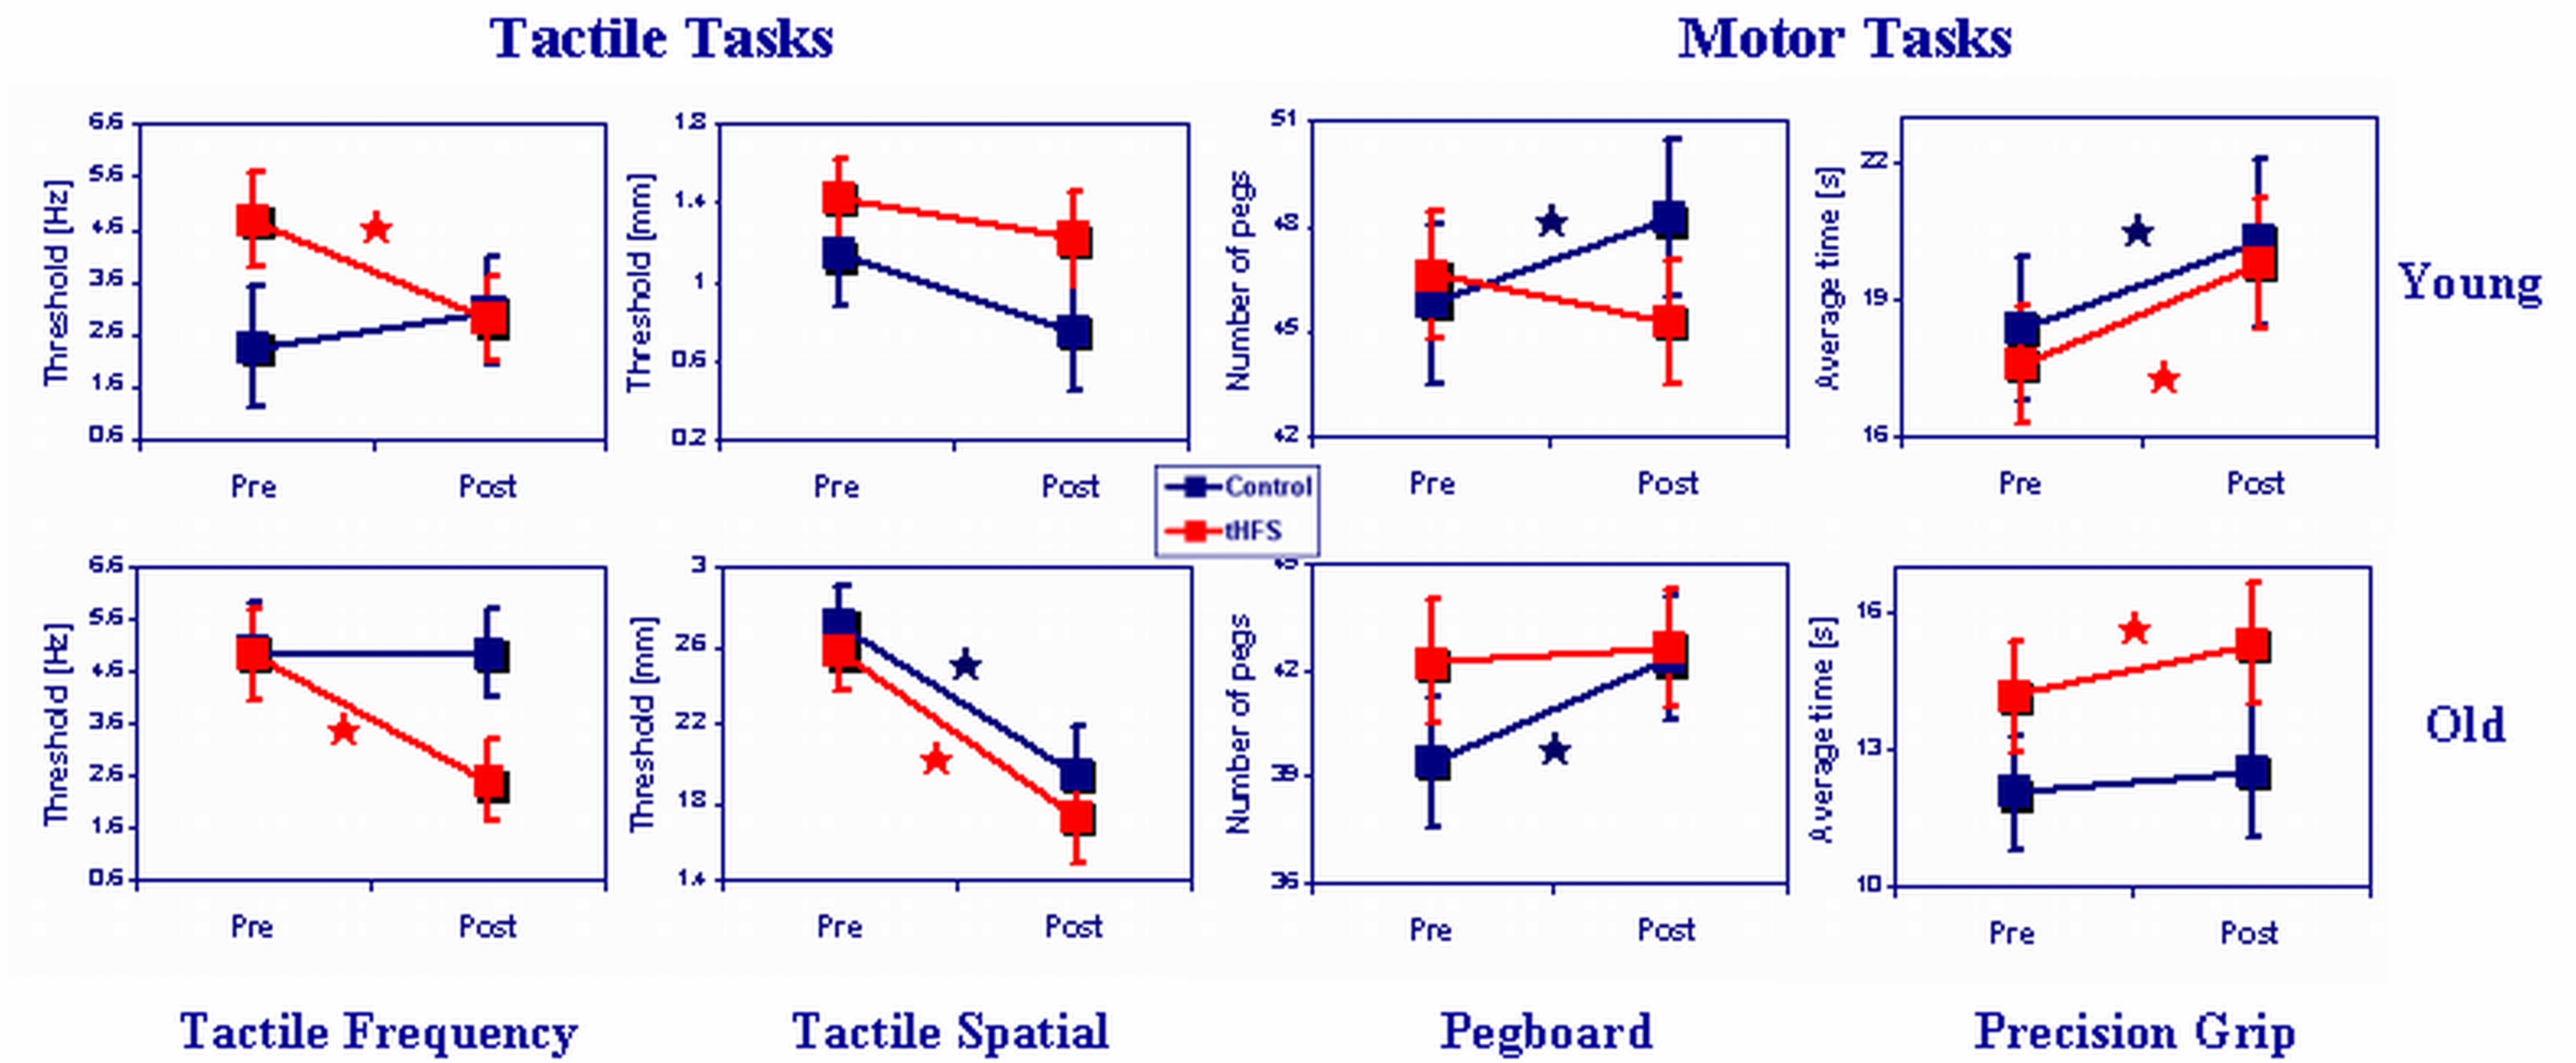
\includegraphics[width=0.5\textwidth]{profBenGodde-fig1}
    \caption{Differential effects of tHFS on tactile (left 2 columns) and motor (right 2 columns) performance in young (top) and old (bottom) subjects. Experimental group shown in red, control group in blue.}
    \label{fig:profBenGodde}
  \end{center}
\end{figure}




\enlargethispage*{0.2cm}
\paragraph{Collaborations}
\begin{itemize}
\item University Hospital T\"{u}bingen \\ MEG-Center \\ PD Dr. Christoph Braun 
\item University of T\"{u}bingen \\ Medical Psychology and Behavioral Neurobiology \\ Dipl-Psych. Ahmed A. Karim
\item International School for Advanced Studies \\ Trieste, Italy \\ Cognitive Neuroscience Sector \\ Prof. Mathew E. Diamond, PhD
\item Lerner Research Institute, USA \\ Department of Biomedical Engineering \\ Cleveland Clinic Foundation \\ Jay L. Alberts, PhD
\item IUB, SES \\ Prof. Dr. Claus Hilgetag
\item University of Bremen \\ Interdisciplinary Center for Cognitive Sciences \\ Prof. Dr. Manfred Herrmann; Prof. Dr. Manfred Fahle
\end{itemize}

\begin{bibunit}[apalike]
\nocite{*}
\putbib[profBenGodde1]
\end{bibunit}

\paragraph{Grants}
\begin{itemize}
\item DFG (submitted; PI: C. Voelcker-Rehage in cooperation with Jay L. Alberts, PhD, Cleveland Clinic Foundation, USA): Age-related changes in functional uni- and bimanual dexterity; grasping force modulation in older adults.

\item BMBF (PI: JCLL). B. Godde, C. Voelcker-Rehage: subproject ``Adaptive Competence'' within the joint research project ``Effects of Matches/Mismatches between Aspects of Human and Social Capital, Corporate Strategy and Work Organization on the Physical and Mental Well-Being of Employees''. 
 
\end{itemize}

\subsection{Effects of Cardiovascular and Motor Fitness on Cognitive Performance and Well-Being in Older Adults}


\index{Godde, Ben}

\paragraph{Research Team}
Claudia Voelcker-Rehage (Postdoctoral Fellow), Ben Godde (Professor), Ursula M. Staudinger (Professor), Mikhail Babanin (Doctoral Fellow), Kathrin Linke (Diploma Student), Tanja Truhart (Student, University Bremen), Silja Menken (Student, University Marburg), Pit Peltz (Student, University Bremen).

Following an interdisciplinary view on human performance that comprises motor, neurophysiological and psychological expertise and methods, our second area of research deals with the role of cardiovascular fitness and motor coordination training on cognitive performance and psychological well-being in older adults. More and more animal and human studies stress the importance of a physically active lifestyle for successful aging (i.e. retarded cognitive decline, improved physiological and psychological health etc.). However, the underlying mechanisms, the dose-response-relationship and also the effects of different types of exercise on cognitive performance are still not well understood.

\null
\textbf{Research Highlights 2006}

 Currently we are performing a one-year longitudinal study to investigate the effect of different types of physical activity on cognitive performance and well-being in older adults. 
\newpage 
This study started in October 2006 and results of baseline measurement are just under investigation. In preliminary studies we developed and evaluated training programs and test batteries for practicing and assessing gross and fine motor coordination in older adults. We also performed a pilot cross sectional study on the effects of different types of physical exercise (endurance training, strength training, mixed training) on cognition and well-being. 

\begin{figure}[h]
  \begin{center}
    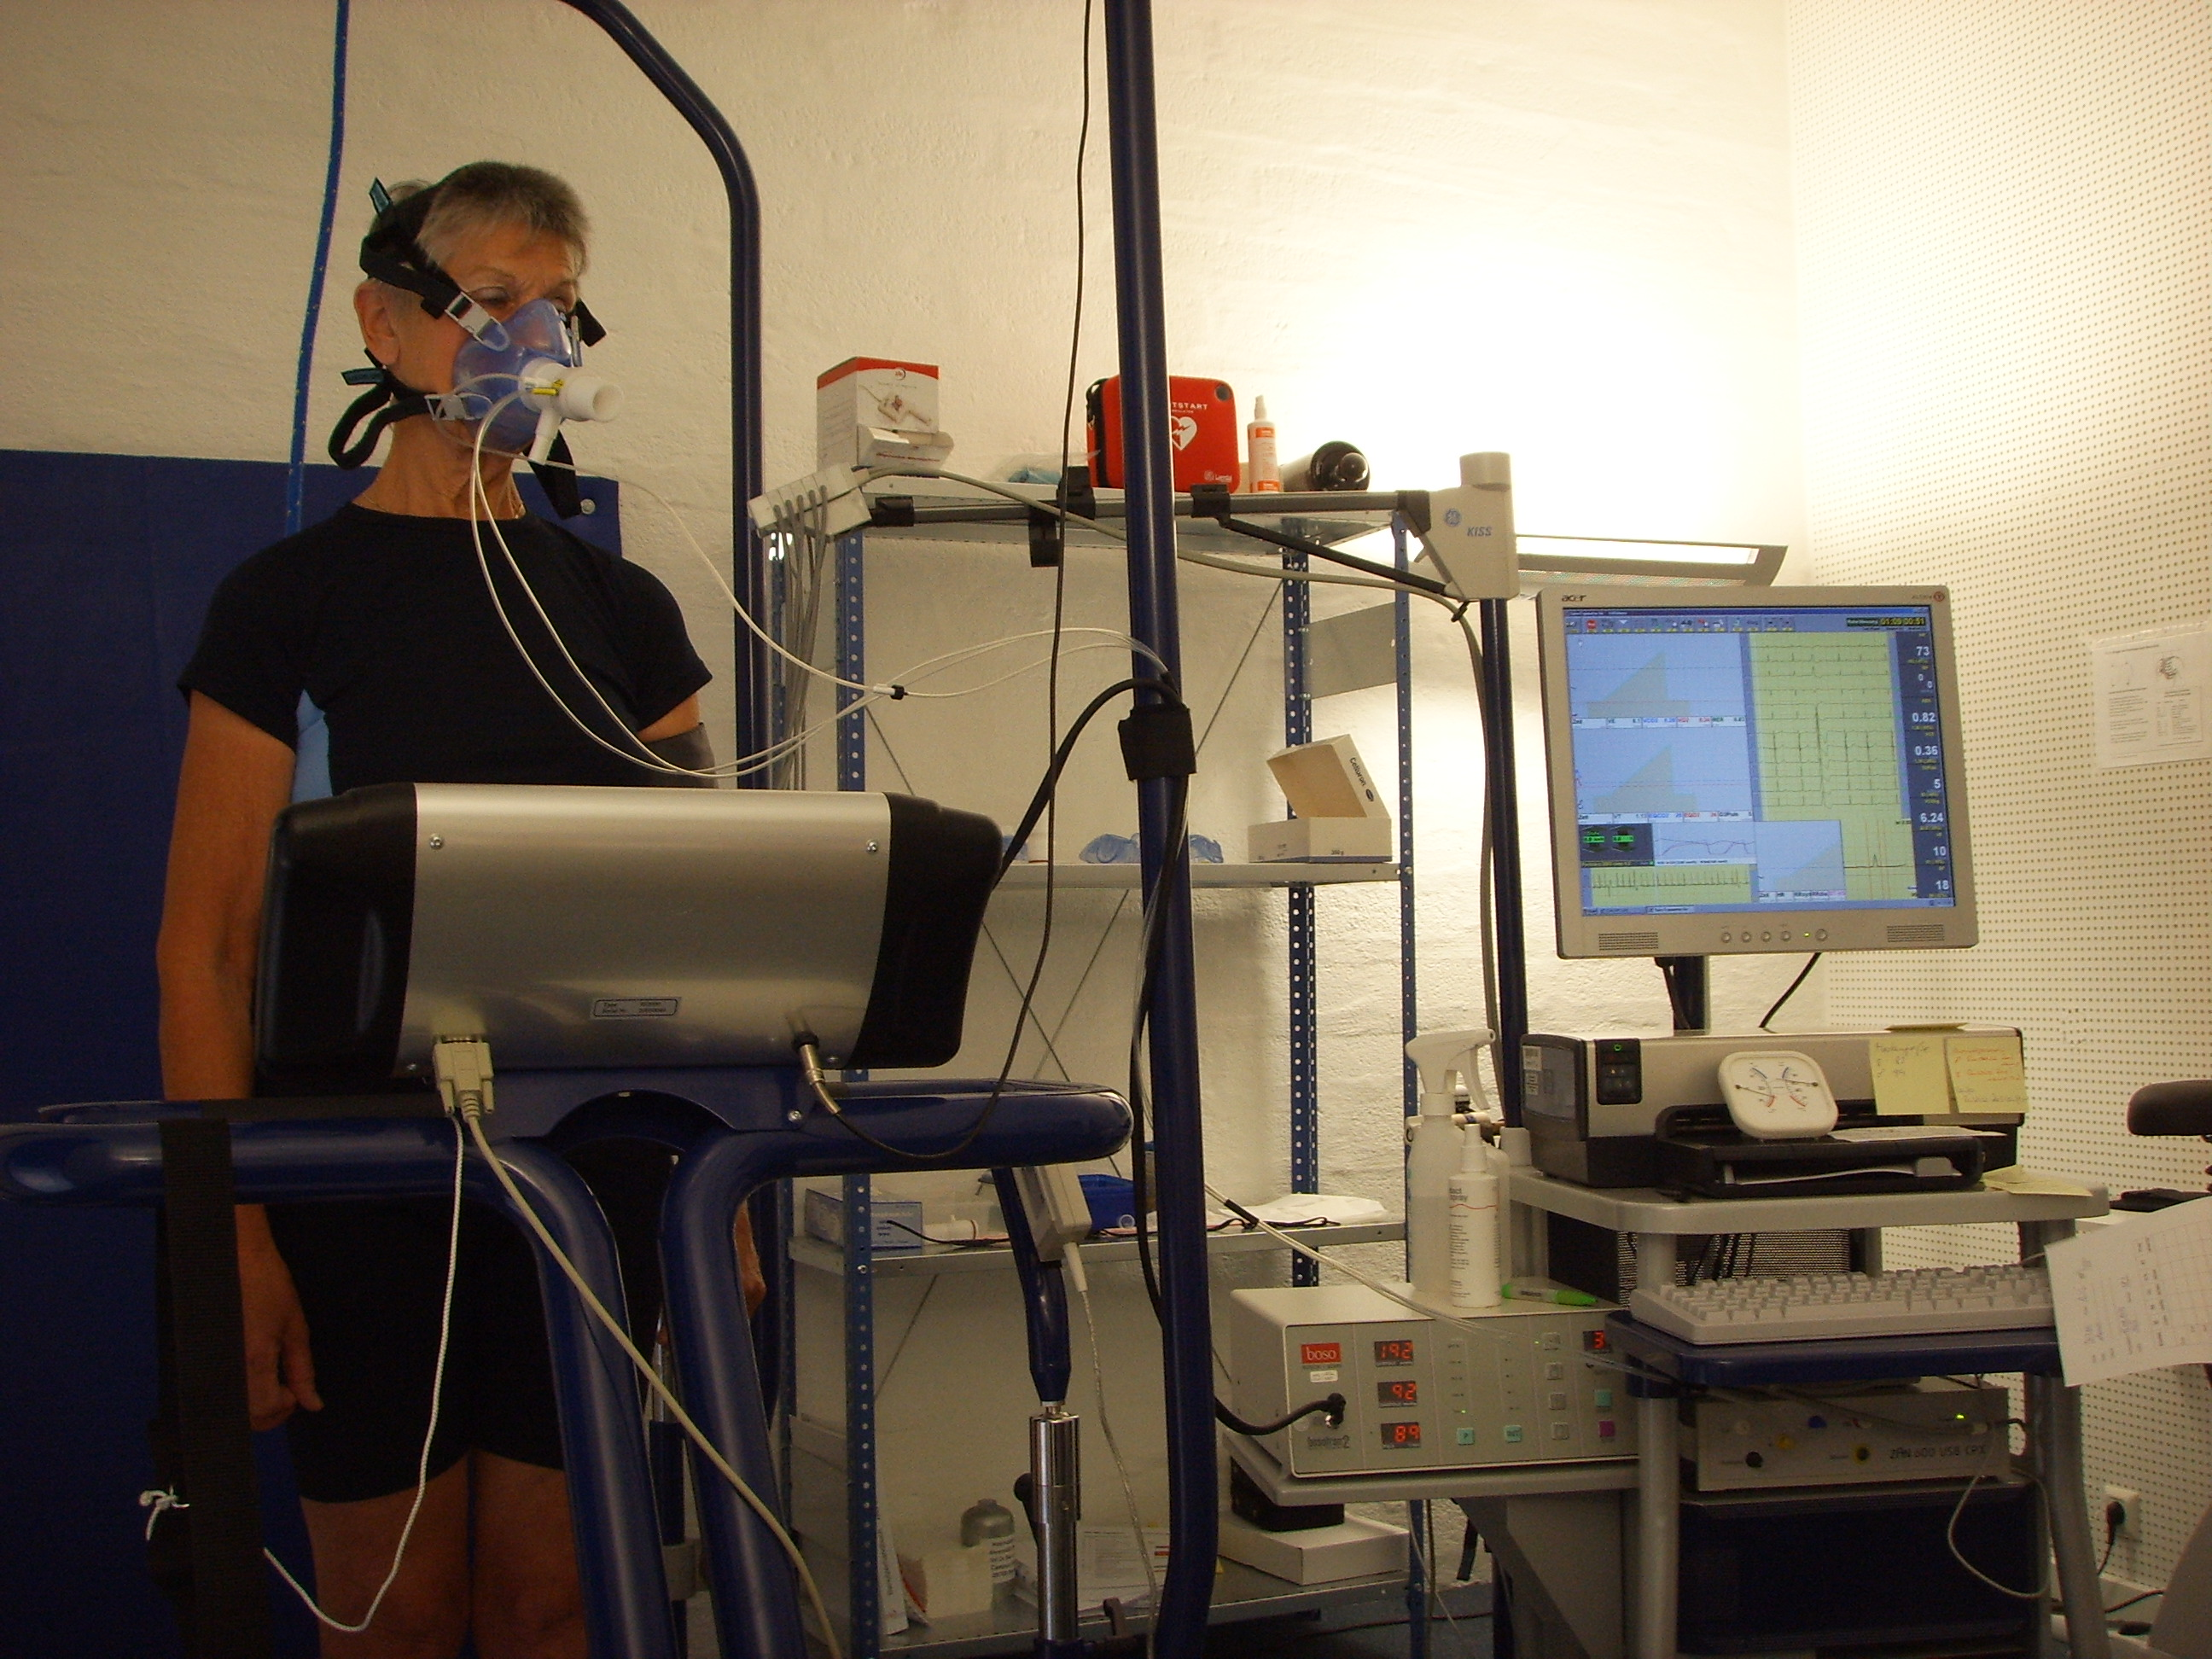
\includegraphics[width=7.5cm]{profBenGodde-fig2.jpg}
    \caption{Using a ZAN600 spiroergometric system (ZAN Messtechnik, Oberthulba, Germany) we measure the cardiovascular and respiratory fitness of participants to develop individual recommendations for their training programs.}\label{fig2:profBenGodde}
   \end{center}
\end{figure}

\textbf{Collaborations}
\begin{itemize}
\item University of Bielefeld \\ Department of Sports Science \\ Prof. Dr. Klaus Willimczik
\item University of Bremen \\ Movement Science and Training\\ Sports Science \\ Dr. Monika Fikus
\item University of Bremen \\ Interdisciplinary Center for Cognitive Sciences \\ Prof. Dr. Manfred Herrmann
\item IUB, JCLL \\ Prof. Dr. Ursula M. Staudinger
\end{itemize}

\begin{bibunit}[apalike]
\nocite{*}
\putbib[profBenGodde2]
\end{bibunit}

\paragraph{Grants}
\begin{itemize}
\item Robert Bosch Foundation \& German Health Insurance Company (PI: C. Voelcker-Rehage in cooperation with B. Godde and U.M. Staudinger, JCLL, IUB): Facilitating Motor and Cognitive Performance in Old Age.
\item DFG travel grant for C. Voelcker-Rehage, Society for Neuroscience Annual Meeting, October 14-17, 2006, Atlanta, GA, USA.
\item DFG travel grant for C. Voelcker-Rehage, Annual meeting of the North American Society for Psychology of Sport and Physical Activity, June 9-11, 2006, St. Petersburg Beach, FL, USA.
\end{itemize}





\subsection{Awards, Fellowships}

\begin{itemize}
\item Junior Fellow of the Leopoldina-Acatech Working group ``Chancen und Probleme einer alternden Gesellschaft: Die Welt der Arbeit und des lebenslangen Lernens'' (Claudia Voelcker-Rehage).
\end{itemize}
 
\subsection{Other Professional Activities}

\textit{Ad-hoc Reviews}

\begin{itemize}
\item Godde, B.: \\Journal of Cognitive Neuroscience; Cognition; Quarterly Journal of Experimental Psychology, Journal of Neuroscience, Neuroscience and Biobehavioral Reviews; Experimental Brain Research; Journal of Neuroscience Methods; ACM Transactions on Applied Perception; Behavioural Brain Research.
\item Voelcker-Rehage, C.: \\European Review of Aging and Physical Activity.
\end{itemize}



\cleardoublepage
\section{A View on Lifelong Learning from Health and Personality
Psychology} \shorttitle{Health and Personality
}
\subsection{Health Psychology}

\index{Renner, Britta}

\paragraph{Research Team}
Britta Renner (Professor), Youlia Spivak (Doctoral Fellow), Andries Oeberst (Doctoral Fellow), Martina Panzer (Doctoral Fellow).

 The Health Psychology Research Group is interested in the judgment and decision-making processes that underlie the onset, maintenance, and cessation of health-relevant behaviors with a particular emphasis on risk perception and reactions towards risk information. The activities of our research group are designed to further the synthesis of basic research on how people process and utilize health information and whether there are age-related differences in the functionality of health behavior changes. These efforts are motivated by the broader goal of developing theoretical frameworks that can be applied across a range of behavioral domains.

\null
\textbf{Research Highlights 2006}

 The DFG-funded longitudinal research project ``Risk Appraisal Consequences in Korea'' (RACK) is conducted in Seoul, South Korea, in collaboration with Prof. Dr. Ralf Schwarzer at the Free University of Berlin, Prof. Sunkyo Kwon at the Sookmyung University, Prof. Dr. Byung-Hwan Yang at the Hanyang University, and Prof. Dr. Ki-Chung Paik at the Dankook University (N = 1359). The research project focuses on the effects of individualized health feedback on health-related cognitions and health behavior changes in various age groups. This project is unique in its scope because for the first time the health behavior change process will be examined from a psychological perspective and can be compared directly to a western sample. See also http://www.gesundheitsrisiko.de/.

\newpage
\textit{Processing and Impact of Self-Relevant Risk Communication in Adulthood}

 At first glance, perceiving a health threat seems to be the most obvious prerequisite for the motivation to change risk behaviors. If one is not aware of the risky nature of one's actions, motivation for change cannot emerge. Therefore, a crucial barrier that health communication needs to overcome in order to be effective is to focus people's attention on information that pertains directly to their personal risk, thereby increasing the personal relevance of a health issue (Renner, Panzer, \& Oeberst, in press; Renner, Sch\"{u}z, \& Sniehotta, submitted; Renner \& Schwarzer, 2000, 2003; Renner \& Schupp, 2005; Weinstein, 1998, 2003). However, numerous empirical studies demonstrate differential acceptance of negative and positive risk information (cf. Croyle, Sun, \& Hart, 1997).

\enlargethispage*{0.5cm}

 Most researchers interpret these findings as evidence for motivated reasoning, arguing that people- who are informed that they have an elevated risk of disease minimize the seriousness of the health threat posed by the risk information and derogate the validity of the risk factor test in order to maintain a favorable sense of their health. However, the assumption of motivated reasoning has been challenged by the ``cue adaptive reasoning account'' (CARA; Renner, 2004). Extending the CARA research design introduced by Renner (2004), the present project focuses on the processing of self-relevant risk feedback (total cholesterol, blood pressure) in order to gain a more in-depth understanding of how people react towards risk communication. Moreover, the research project examines how reactions towards self-related risk feedback are related to age. This research is expected to provide particularly important information regarding effective risk communication. Analyses of spontaneous reactions toward blood pressure feedback show in accordance with the CARA approach that feedback valence and feedback expectedness are central processing categories.

\newpage
\textit{Health Cognitions and Health Behaviors}

 Engagement in preventive health behaviors is not merely determined by the awareness of objective health risks but it is mainly influenced by health beliefs and specific health cognitions (Renner \& Schwarzer, 2003, 2005). The goal of the research project based on data from the ``Risk Appraisal Consequences in Korea'' (RACK) and Berlin Risk Appraisal and Health Motivation Study (BRAHMS) is to further the development of current health models, in particular the Health Action Process Approach (HAPA; Renner \& Schwarzer, 2003; 2005; Renner, Yang, Paik, Kim, Roh, Song, \& Schwarzer, in press; Schwarzer, 1999; Schwarzer \& Fuchs, 1996). HAPA is regarded as a heuristic to better understand the complex mechanisms that operate when people become motivated to change their behavior, and when they attempt to resist temptations. It applies to all health-compromising and health-enhancing behaviors and pays particular attention to postintentional mechanisms, and it conveys an explicit self-regulation perspective. Four areas of health behavior are the focus of the study: Nutrition, physical activity, smoking, and alcohol consumption. First results for nutrition confirm the predictive power of the Health Action Process Approach but point to the role of gender in the self-regulation of dietary behaviors (Renner et al., in press; see Figure \ref{fig2:profBrittaRenner}).

\begin{figure}[h!tb]
  \begin{center}
    \resizebox{0.5\textwidth}{!}{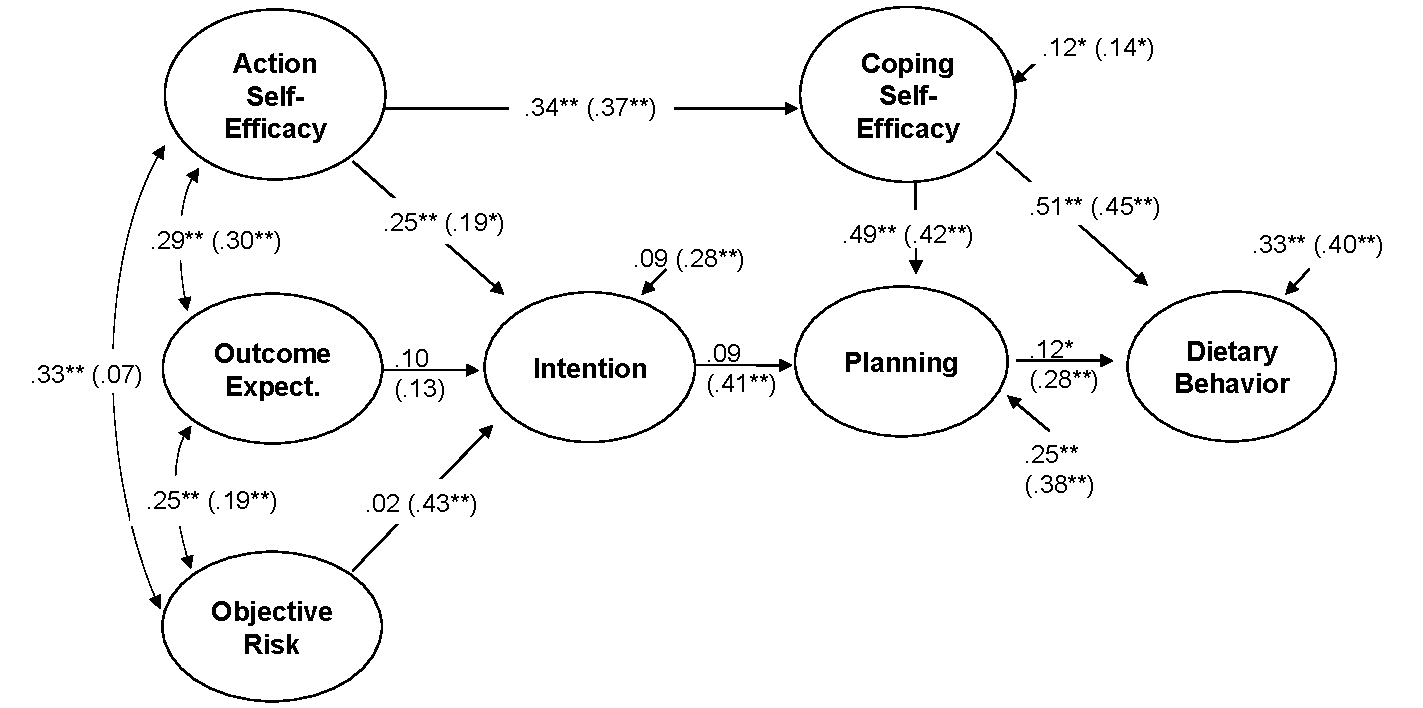
\includegraphics{profBrittaRenner-fig2}}
    \caption{Two-group prediction model for dietary behaviors in South Korean men and women. Coefficients for women in parentheses. (Renner et al., in press.)}
    \label{fig2:profBrittaRenner}
  \end{center}
\end{figure}


\newpage
 To date, little is known about how determinants of the process of health behavior change vary across the lifespan. Social cognition models of health behavior are commonly understood as being universal, implying that they are applicable to groups that vary, for example, in age or cultural background. Cultural uniqueness and specific characteristics of lifespan development, however, necessitate the study of differential effects. For instance, previous research suggests that with increasing age, risk perception becomes a more important motivational drive even though the actual health status may have not changed (Renner, Knoll, \& Schwarzer, 2000; Schwarzer \& Renner, 2000).

 Therefore, the present research project also examines whether there are age-related differences in health-related cognitions, health behaviors, and the functionality of health behavior changes. These efforts are motivated by the broader goal of developing theoretical frameworks that can be applied across a range of behavioral domains.

 Accordingly, the Health Action Process Approach is examined in younger and middle-aged/older adults from South-Korea who participated in a longitudinal health screening study with a 6-month time lag. First results suggest a different motivation for the involvement in physical activity as a function of age (Renner, Spivak, Kwon, \& Schwarzer, submitted).

{\textit{Health-Related Behavior, Risk Perception, \& Risk Stereotypes}

 Extending previous research, this research project examines not only what people consider as risky (high risk stereotype) but also what they consider as safe (low risk stereotype). This approach allows testing the hypothesis that it is the ratio of the low risk stereotype, the self, and the high risk stereotype which determine risk perception (Renner \& Schwarzer, 2003; Renner \& Schupp, 2005). Part of the research program examines whether low and high risk stereotype images are related to risk perceptions and, in particular, to unrealistic optimism. Particularly, we investigate whether people actively construe images of low and high risk stereotypes in order to maintain a favourable standing in comparison to others.

 The second goal of this project which is conducted in cooperation with the University of Konstanz and funded by the DFG is to examine the effects of risk stereotypes and of affect on risk perceptions in the domain of HIV and sexually transmitted diseases. This research project incorporates four new aspects: (1) devising a new method to assess self-related risk perceptions which enables identifying unrealistically optimistic risk perceptions at the individual rather than at the group level; (2) examining the role of stereotypical beliefs about persons that are high or low at risk (risk stereotypes) for self-related risk perceptions; (3) examining the role of affect for other-related risk perception from a multi-system perspective including established neuroimaging and psychophysiological measures; and (4) assessing the interplay of self-related and other-related risk perceptions. Exploring these issues is considered relevant for a better understanding of the knowledge-behavior gap, i.e. the comparably low prevalence of protective behavior despite high knowledge about health risks. In the long run, this research will contribute towards the overarching goal of devising more effective risk interventions called for by the World Health Organization and other health expert institutions.


\paragraph{Collaborations}
\begin{itemize}
\item Free University of Berlin \\ Prof. Dr. Ralf Schwarzer 
\item Sookmyung University, South Korea \\ Prof. Dr. Sunkyo Kwon
\item Hanyang University, South Korea \\ Prof. Dr. Byung-Hwan Yang
\item Dankook University, South Korea \\ Prof. Dr. Ki-Chung Paik
\item University of Konstanz \\ Prof. Dr. Harald Schupp 
\item KTL Public Health Institute Helsinki \\ Dr. Pilvikki Absetz
\item Charit\'e Berlin \\ Prof. Dr. Claudia Spies; Dr. Birte Dohnke; Dr. Edith Weiss-Gerlach; Dr. Andrea Mossner
\item Universidad Estatal a Distancia San Jos\'e \\Dr. Benicio Guti\'errez-Do\~na
\end{itemize}

\begin{bibunit}[apalike]
\nocite{*}
\putbib[profBrittaRenner1]
\end{bibunit}


\paragraph{Grants}
\begin{itemize}
\item DFG Re1583/2-1 (PI: B. Renner in cooperation with R. Schwarzer, Free University Berlin): Individualized Feedback after Blood Pressure and Cholesterol Screenings: The Role of Health Beliefs, Health Behaviors, and Actual Health Status.  
\item DFG RE 1583/3-1  (PI: B. Renner in cooperation with H. Schupp, University of Konstanz): Self-Related and Other-Related Risk Perception: The Impact of Risk Stereotypes and Affective Responses.
\item CONARE-Project, Costa Rica S. No26-06, 01/08/06 (Start: 2007). (PI: B. Renner in cooperation with B. Guti\'errez-Do\~na, Universidad Estatal a Distancia San Jos\'e and R. Schwarzer, Free University Berlin): Individualized Feedback after Blood Pressure and Cholesterol Screenings. 

\item BMBF (PI: JCLL). B. Renner: subproject ``Health Promotion'' within the joint research project ``Effects of Matches/Mismatches between Aspects of Human and Social Capital, Corporate Strategy and Work Organization on the Physical and Mental Well-Being of Employees''. 
\end{itemize}


\subsection{Personality Psychology}

\index{Renner, Britta}

\paragraph{Research Team}
Britta Renner (Professor), Freda-Marie Hartung (Doctoral Fellow).

 A first line of research of the Personality Psychology Research Group focuses on interpersonal perception with a particular emphasis on expectancies and curiosity. The goal of this line of research is to determine how people derive judgments of another person, which factors facilitate or diminish the accuracy in personality judgments and how accuracy varies with age. 
A second line of research focuses on the conceptualizing of and reaction towards optimism, pessimism, and realism. Numerous studies have demonstrated that optimism is linked to positive outcomes (e.g., health) by a ``social pathway'' (Peterson \& Bossio, 2001). However, this \
``social pathway'', that is social reactions towards optimism and pessimism, has only rarely been studied. Therefore, the goal of this line of research is to examine whether judges respond differentially to optimism, realism and pessimism, and whether these differential responses can be related to specific cues of optimism, realism and pessimism.

\null
\textbf{Research Highlights 2006}

{\textit{Development of a Measurement of Social Curiosity in Adults}

 Curiosity refers to the desire for acquiring new information. Available measures assess curiosity predominantly in the non-social domain. The aim of the present study was to develop a questionnaire to assess social curiosity, i.e., interest in how other people think, feel and behave. The questionnaire was administered to 312 participants. Factor analyses of the 10-item Social Curiosity Scale (SCS) yielded two factors: (1) General Social Curiosity and (2) Covert Social Curiosity. Evidence of convergent validity was provided by moderately high correlations of the SCS with other measures of curiosity and self-perceived curiosity, while divergent validity was demonstrated by low correlations of the SCS with other personality traits, such as neuroticism and agreeableness. Interestingly, social interaction anxiety was observed to facilitate covert social curiosity while inhibiting general social curiosity (cf., Renner, 2006). Taking a lifelong learning perspective, we were additionally interested in the question, how curiosity or the motivation to learn about our physical and social world varies across the lifespan. In contrast to common stereotypes, curiosity did not decrease with increasing age suggesting that the basic motivation to learn appears to remain stable over the lifespan.

\textit{Conceptualizing of and Social Reaction towards Optimism, Pessimism and Realism}

 Numerous studies have shown that optimism is linked to positive outcomes (e.g., health) by a ``social pathway'' (Peterson \& Bossio, 2001). This research program focuses on the question how lay people perceive typical optimistic, pessimistic and realistic acts (DFG funded research project together with Prof. Dr. Hannelore Weber, University of Greifswald). Using a multidimensional perspective, not only typical behavior and typical thoughts are assessed but also typical feelings and typical goals are considered from an act frequency perspective (Weber, Vollmann, \& Renner, in press). In a second step, this line of research examines reactions to optimistic, realistic and pessimistic prototypical acts. Specifically, two experiments (N = 240 and N = 120) examined social responses toward optimists, pessimists, and realists (Vollmann, Renner, \& Weber, submitted). Participants listened to tape-recorded conversations in which optimistic, pessimistic and realistic targets reported how they were dealing with a stressful situation before completing a questionnaire assessing (a) their evaluation of the target's behavior and personality, (b) their attraction to the target, and (c) their willingness to provide the target with social support. Optimistic and realistic targets were viewed more favorably than pessimistic targets, while the behavior of realists was regarded as being more adequate than that of optimists. However, the more positive evaluation of optimists and realists compared to pessimists was not accompanied by a greater willingness to provide them with social support (see Figure \ref{fig3:profBrittaRenner}). The unequivocally high willingness to provide support to both optimists and pessimists might suggest that optimists are in fact not provided with more social support than pessimists. Accordingly, the greater availability of social support commonly reported by optimists (e.g., Brissette et al., 2002) might represent an optimistically biased perception rather than an accurate reflection of the support they are provided with.

\begin{figure}[ht]
  \begin{center}
    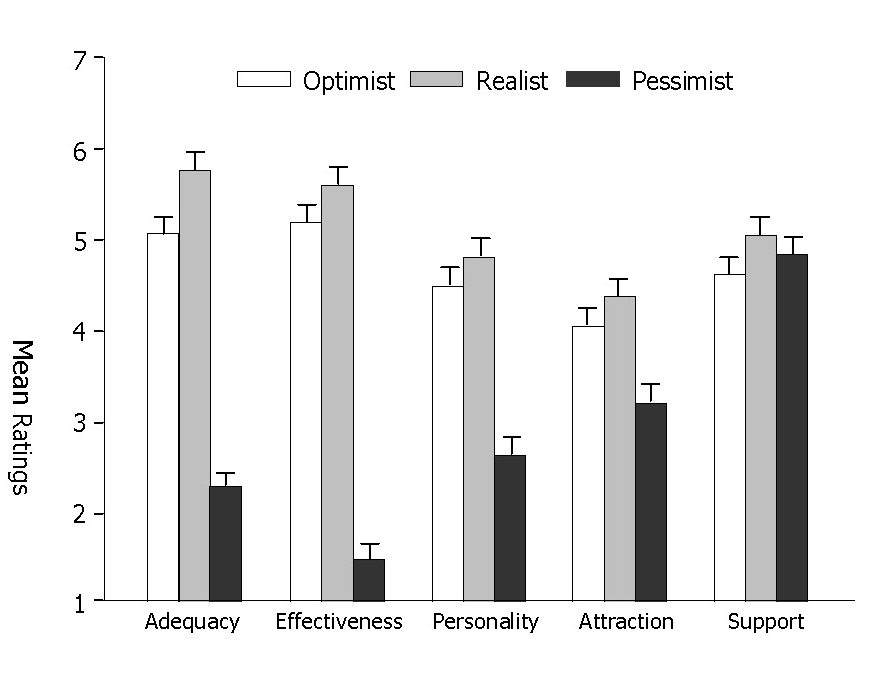
\includegraphics[height=25ex, width=0.5\textwidth]{profBrittaRenner-fig3.jpg}
    \caption{Mean evaluation ratings (with standard errors) of the target as a function of the type of target behavior pattern (Study 2). Note: Higher values indicate a more positive evaluation. (Vollmann, Renner, \& Weber, submitted)}\label{fig3:profBrittaRenner}
   \end{center}
\end{figure}


\textbf{Collaborations}
\begin{itemize}
\item University of Greifswald \\ Prof. Dr. Hannlore Weber; Dipl.-Psych. Manja Vollmann
\item University of Halle \\ Prof. Dr. Peter Borkenau
\end{itemize}

\enlargethispage{1cm}
\begin{bibunit}[apalike]
\nocite{*}
\putbib[profBrittaRenner2]
\end{bibunit}

\subsection{Other Professional Activities}

\begin{itemize}
\item President of the European Health Psychology Society (EHPS).
\item Chair of the Scientific Committee of the 20th Conference of the European Health Psychology Society in Warsaw, 2006.
\item Organizer of the Summer School of the Fachgruppe Gesundheitspsychologie der Deutschen Gesellschaft f\"{u}r Psychologie, International University Bremen, JCLL, Bremen, 2006.
\item Member of the Scientific Committee of the Fachgruppentagung Gesundheitspsychologie, Deutsche Gesellschaft f\"{u}r Psychologie, 2007.
\item Expert for the subject area ``risk perception and behavior'', Division of Health Psychology of the Deutsche Gesellschaft f\"{u}r Psychologie.
\end{itemize}

\textit{Editorial Board Memberships}

\begin{itemize}
\item European Health Psychology Review.
\item	Zeitschrift f\"{u}r Gesundheitspsychologie (Journal of Health Psychology).
\end{itemize}

\textit{Ad-hoc Reviews}

\begin{itemize}
\item Cognition and Emotion; Diagnostica; European Journal of Personality; Experimental Psychology; Journal of Individual Differences; Journal of Positive Psychology; Journal of Public Health; Memory; Psychology \& Health; Psychology, Health \& Medicine; Social Cognition; Social \& Preventive Medicine; Social Science \& Medicine; Zeitschrift f\"{u}r Gesundheitspsychologie.
\item Reviewer for DFG.
\end{itemize}
 
 


\cleardoublepage
\section{The Mechanics and Pragmatics of Lifespan Development: Conceptualization, Measurement and Plasticity}
\shorttitle{Mechanics and Pragmatics of Lifespan Development}

According to modern notions of development such as the lifespan approach, human development is the result of the interaction between three different sources: biology (maturation/senescence), culture (learning), and an individual (decision/action). It is further assumed that psychological phenomena can be meaningfully and for heuristic purposes distinguished in those of the life mechanics and those of the life pragmatics (e.g., Staudinger \& Pasupathi, 2000). Life mechanics reflect individual differences in biology-based patterns of perception, information processing, emotion, and motivation (e.g., basic motivational (approach/avoidance) and emotional (positive/negative) patterns, temperament, speed of information processing, executive processes). Life pragmatics reflect individual differences in the accumulated and constructed experiences with the world (i.e., other people, events, circumstances, rules, places, and objects relevant for leading our lives) and with our self, as well as ways of dealing with the world and with ourselves (e.g., coping, emotion regulation, goal system). In the long run, it seems essential for our understanding of developmental processes to successfully decipher the co- and interaction of those two elements. Presently our research efforts however concentrate on the domain of life pragmatics. Life pragmatics can be distinguished in constructs related to insight and those related to compository or management strategies. With regard to insight, we study insight into life (life insight) as well as insight into our self (self-insight) and the highest form of both, that is, wisdom. With regard to compository strategies, we are especially interested in personal life investment, emotion regulation, coping and time experience. 

Life insights as well as life-compository structures and processes are not determined but plastic. Within a 'norm of reaction' better or worse developmental trajectories are conceivable. Given this basic contention of the plasticity of human development, it is crucial to determine the conditions of plasticity as well as its limits in different domains of psychological functioning. Thus, a third and fourth research focus concern themselves with the theoretical and empirical investigation of the plasticity of human development. The third focus concentrates on the effects of (in particular social) contexts on adult development and the fourth focus is primarily theoretical in nature. It explores the question of different types of plasticity, such as growth and resilience, and pursues the thesis that it is useful to distinguish two different kinds of positive adult development, one aiming towards growth and the other geared towards adjustment. In the following, these four research foci are described in turn.

\textbf{Central reference} Staudinger, U. M. \& Pasupathi, M. (2000). Lifespan perspectives on self, personality and social cognition. In T. A. Salthouse \& F. I. M. Craik (Eds.), The handbook of aging and cognition (pp. 633-688). Hillsdale, NJ: Erlbaum.

\subsection{Life Insight, Self Insight, and
Wisdom: Measurement, Age Trajectories}


\index{Staudinger, M. Ursula}

\paragraph{Research Team}
Ursula M. Staudinger (Professor), Jessica D\"orner (Doctoral Fellow; graduated 05/2006; postdoctoral fellow until 08/2006).

Life insight, and in particular wisdom as its highest form, represent the prototype of growth in adulthood. One may think that such phenomena defy empirical study. But a reliable and valid measurement paradigm has been developed (Baltes \& Staudinger, 2000). Consistent with cultural-historical writings about wisdom, there is empirical evidence that wisdom is indeed a phenomenon that depends on the successful integration of mind and character (Staudinger, Lopez, \& Baltes, 1997). The analysis and evaluation of important life experiences play an important part in that integration process. Thus, it does not come as a surprise that it is not enough to grow older to become wiser. In the last two years, a differentiation between personal wisdom and self-insight on the one and general wisdom and life insight on the other hand has been introduced and a measurement paradigm has been developed. This distinction is based on the assumption that distinguishable psychological phenomena are concerned when you have to be wise about a problem of your own life or life in general.

\null
\textbf{Research Highlights 2006}

Using the two new measures of self-insight or personality maturity that had been developed before, we started to investigate their age trajectories during the last year. As expected, based on the literature on personality growth, we found that neither self-related wisdom nor self-concept maturity normatively show positive age differences. In terms of self-related wisdom, we even found negative age differences in particular with regard to the three meta criteria of self-related wisdom, that is, tolerance, embeddedness and tolerance of ambiguity. This finding is consistent with the interpretation that the last developmental task of life, that is, integrating our lives and finding peace in the face of human terminality, may be juxtaposed to the goal of pursuing self-related wisdom.

\paragraph{Collaborations}

\begin{itemize}
\item Max Planck Institute for Human Development, Berlin\\ Prof. Dr. Paul B. Baltes ($\dagger$)
\item Oregon State University\\ Prof. Karen Hooker, PhD
\item IUB, JCLL\\ Prof. Dr. Ute Kunzmann
\item IUB, JCLL\\ Prof. Dr. Sven V\"olpel
\item University of Florida, Gainsville, FLA\\ Prof. Manfred Diehl, PhD
\item Universit\"at Frankfurt\\ Prof. Dr. Tilmann Habermas
\item Universit\"at Wien\\ Prof. Dr. Judith Gl\"uck
\end{itemize}

\begin{bibunit}[apalike]
\nocite{*}
\putbib[profUrsulaStaudinger1]
\end{bibunit}

\paragraph{Grants}
\begin{itemize}
\item DFG STA 540/3 -1/2(PI: U.M. Staudinger): Is it possible to promote self-insight? (2001-2005)
\end{itemize}

\subsection{Life Composition: Measurement and Age Trajectories}


\index{Staudinger, M. Ursula}

\paragraph{Research Team}
Team Ursula M. Staudinger (Professor), Eva-Marie Kessler (Doctoral Candidate; graduated 01/2006; postdoctoral fellow), Ines Schindler (Postdoctoral fellow at Utah State University).

This project is interested in processes of developmental regulation during adulthood and old age. Life composition concerns different aspects of self and personality such as emotions, coping, the goal system, and the experience of time. Besides establishing valid measurement for different age groups, we investigate which role these aspects of self and personality play in resilience constellations and the regulation of subjective well-being of old age. 

\null 
\textbf{Research Highlights 2006}

\textit{Personal Life Investment}

 During 2006, work in the area of the goal system (personal life investment, PLI) focused on the distinction between obligatory and optional PLI. PLI is defined as the amount of motivational energy people invest as actions or thoughts in ten central life domains (health, cognitive fitness, hobbies and interests, relationship with friends and acquaintances, sexuality, well-being of relatives, occupation or similar activities, independence, thinking about one's life, death and dying) in order to achieve their personal goals or prevent the loss of prior achievements. Depending on the developmental tasks of a given age period different domains require our obligatory investment and others leave room for optional investments. 

\begin{figure}[htb]
  \begin{center}
    \resizebox{0.4\textwidth}{!}{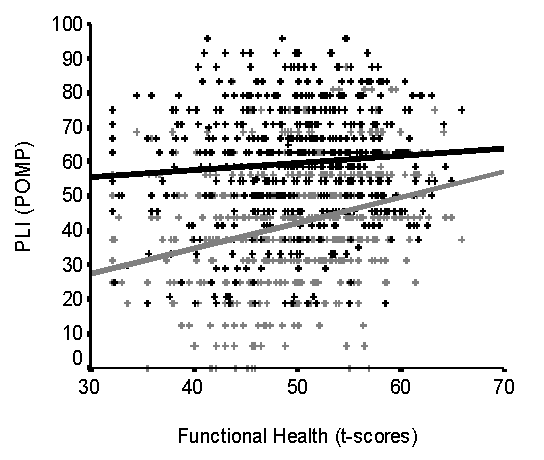
\includegraphics{profUrsulaStaudinger-fig1}}
    \caption{Optional (grey line) and obligatory (black line) as expected differ in their association with levels of objective health. Optional PLI is higher at higher levels of functional health (Schindler \& Staudinger, submitted).}
    \label{fig1:profUrsulaStaudinger}
  \end{center}
\end{figure}


The distinction aims to model the differences between reactive and active types of investments. And indeed, we found that the two types relate differently to indicators of approach and avoidance as well as to indicators of subjective well-being (see Figure \ref{fig1:profUrsulaStaudinger}; Schindler \& Staudinger, submitted). The two types of PLI have demonstrated differential age trajectories in the longitudinal sample of the Berlin Aging Study (Schindler, Staudinger, \& Nesselroade, in press). Across an age range of 30 years and a measurement period of 10 years, optional PLI showed declines and obligatory PLI stayed stable. This finding was replicated when using functional health rather than chronological age as correlate. Obligatory PLI is not related to functional health whereas optional PLI is lower at lower levels of health.

%\begin{figure}[ht]
%  \begin{center}
%    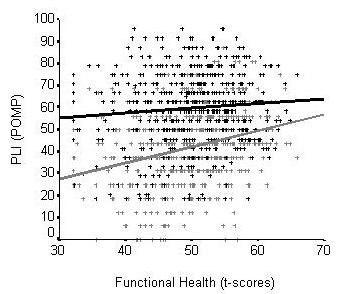
\includegraphics[width=7.5cm]{profUrsulaStaudinger-fig1.png}
%    \caption{Optional (grey line) and obligatory (black line) as expected differ in their association with levels of objective health. Optional PLI is higher at higher levels of functional health (Schindler \& Staudinger, submitted).}\label{fig1:profUrsulaStaudinger}
%   \end{center}
%\end{figure}


Furthermore, in 2006 we conducted a study on the emotional life and its functionality across the lifespan (Kessler \& Staudinger, in preparation). A new emotion questionnaire that assesses the frequency with which certain emotions have been experienced was developed. In contrast to extant questionnaires, the new instrument distinguishes not only between positive and negative emotions but also between emotions that involve high and those that involve low activation. Some of the conflicting patterns of results available in the literature may be related to the lack of this differentiation. And indeed this is what we found: both high and low activated negative emotions decline starting in midlife. Highly activated positive emotions show no age differences, but low activated positive emotions increase starting young adulthood (see Figure \ref{fig2:profUrsulaStaudinger}).

%\begin{figure}[ht]
%  \begin{center}
%    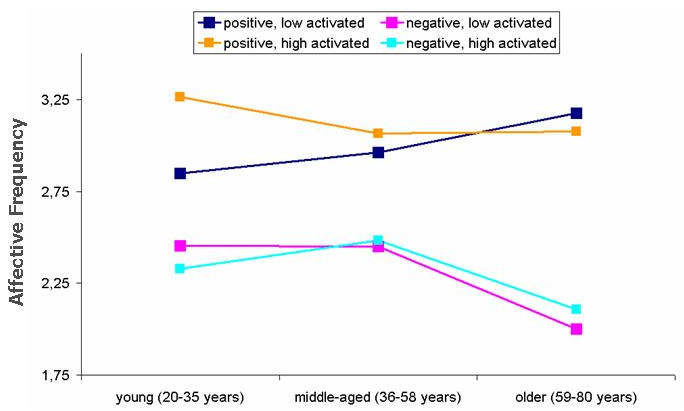
\includegraphics[width=7.5cm]{profUrsulaStaudinger-fig2.png}
%    \caption{Age difference on four facets of emotional life (Kessler \& Staudinger, in preparation).}\label{fig2:profUrsulaStaudinger}
%   \end{center}
%\end{figure}


\begin{figure}[htb]
  \begin{center}
    \resizebox{0.5\textwidth}{!}{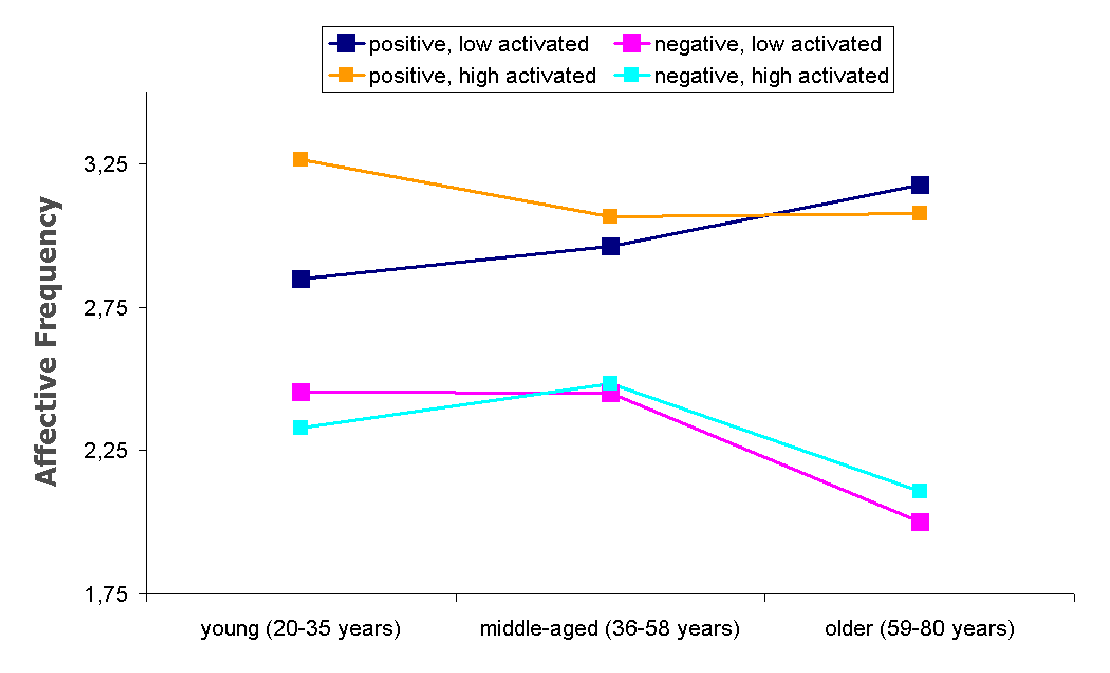
\includegraphics{profUrsulaStaudinger-fig2}}
    \caption{Age difference on four facets of emotional life (Kessler \& Staudinger, in preparation).}
    \label{fig2:profUrsulaStaudinger}
  \end{center}
\end{figure}

\newpage
\paragraph{Collaborations}

\begin{itemize}
\item Brandeis University\\ Prof. Margie Lachman, PhD
\item Stanford University\\ Prof. Laura Carstensen, PhD
\item University Hildesheim\\ Prof. Dr. Werner Greve
\item University of Utah\\ Dr. Ines Schindler
\end{itemize}

\begin{bibunit}[apalike]
\nocite{*}
\putbib[profUrsulaStaudinger2]
\end{bibunit}

\subsection{Context as a Facilitator of Adult Personality
Development}


\index{Staudinger, M. Ursula}

\paragraph{Research Team}
Ursula M. Staudinger (Professor), Heike Heidemeier (Postdoctoral Fellow (since 03/2006), Eva-Marie Kessler (Doctoral Fellow, graduated 01/2006; now Postdoctoral Fellow), Andrea M\"uhlig-Versen (Doctoral Fellow), Martin Noack (Doctoral Fellow since 03/2006).


As mentioned in the Introduction, the plasticity of human development is the third research focus besides the study of life insight and life composition. Plasticity of human development is based on resources. Internal (biological, psychological) and external (contextual) resources can be distinguished. In the present project we are concerned with four different approaches to the study of contextual effects on human development: (1) interactive minds: the facilitative effects of social context; (2) social context and intergenerational potential; (3) activating contexts for old age: the sample case of civic engagement; and (4) the investigation of the effects of the work context on adult development.

\null
\textbf{Research Highlights 2006}

\textit{Interactive Minds}

 In earlier studies on life insight, we had found that under specific conditions (natural partner, time to think after interaction) social interaction facilitates life insight and wisdom (Staudinger \& Baltes, 1996). Furthermore, life-reflection has been identified as a central mechanism in the accumulation of life experience (Staudinger, 2000). We conducted an intervention study that aimed to facilitate self-insight or personality maturity by learning a social-cognitive strategy of how to think about oneself in the present, the past and the future. This strategy is called life-reflection is composed of three elements: (1) remembering experiences, (2) explain experiences, (3) evaluate experiences in the context of one's life. Based on earlier work on interactive minds (Staudinger \& Baltes, 1996), we recruited natural dyads to come to the lab. These dyads were randomly assigned to the following experimental conditions: (1) Life reflection dyad, (2) Life reflection alone, (3) Reminiscence, (4) Thinking time alone. In each of the conditions, participants had to respond to a self-related wisdom task (e.g., how are you as a friend?) either with or without having learnt how to do life reflection and either doing it alone or as a twosome. First results with regard to the new measure of self-related wisdom showed that applying the social-cognitive strategy of life reflection increased self-insight significantly. No significant differences between young and old adults were found neither were there differences between the monadic and the dyadic condition. The lack of a facilitative effect of the natural dyadic condition is in contrast to earlier findings with general wisdom. This finding is consistent with the interpretation that conversational partners that know each other well may not be so helpful when it come to stimulating new self-insight, as mutual perceptive patterns have been established as well as tabu topics to be avoided. The study underscores the importance of the social-cognitive process of life reflection on our way to wisdom (Staudinger, D\"orner, \& Mickler, in preparation).

\textit{Social Context and Intergenerational Potential}

 In this study, funded by the DFG, we investigated the effect of age-heterogeneous interactions between adolescents and older adults on psychological functioning (e.g., fluid intelligence, prosocial behavior). The thesis is that the developmental motivations of adolescents (identity formation/information search) and older adults (generativity) provide for a motivational match that facilitates psychological functioning. For this match to be realized, however, the situational conditions need to be such that both motivations get activated. This hypothesis was confirmed. Older adults that interacted with an adolescent over a difficult life problem (that makes the older person the expert) afterwards show higher levels of cognitive functioning on speed-dependent measures than older adults that interacted with adolescents over a new technology problem (that makes the adolescent the expert; Kessler \& Staudinger, submitted). The assumption was that the motivational match would create a motivational boost that activated in particular those aspects of cognitive functioning that are dependent on cognitive energy such as speed measures. In turn, adolescents in age-heterogeneous interaction over a life problem showed significantly more prosocial behavior than those who had interacted with a peer or with an older adult over a technology problem. 

\textit{Contexts that Activate in Old Age: The Sample~Case of Civic Engagement}

 Funded by the BMFSFJ, we conducted a quasi-experimental longitudinal field study that investigated whether the participation in a special volunteer program (EFI) that combines participation in a preparatory training for volunteering with civic engagement leads to personality changes in older adults. The training program aims to develop a role identity in the area of civic engagement and to teach competences necessary in the realm of civic engagement. The EFI participants were compared with a strict control group of older adults that were also active as volunteers but did not participate in this particular program and the seminar. Two types of personality development were stimulated in association with the EFI participation. The first is social adjustment. We found that EFI participants' subjective well-being significantly increased between T1 and T2 and stayed stable between T2 and T3. In contrast the volunteering control group neither showed increases between T1 and T2, nor between T2 and T3. The second positive development was personality growth. However, growth was only found for certain participants. Only, participants high on internal control beliefs showed increases in Openness to Experience (a personality characteristic that usually show age-related decline) between T1 and T2 and continued to grow between T2 and T3 (see Figure \ref{fig3:profUrsulaStaudinger}).

\begin{figure}[h]
  \begin{center}
    \resizebox{0.45\textwidth}{!}{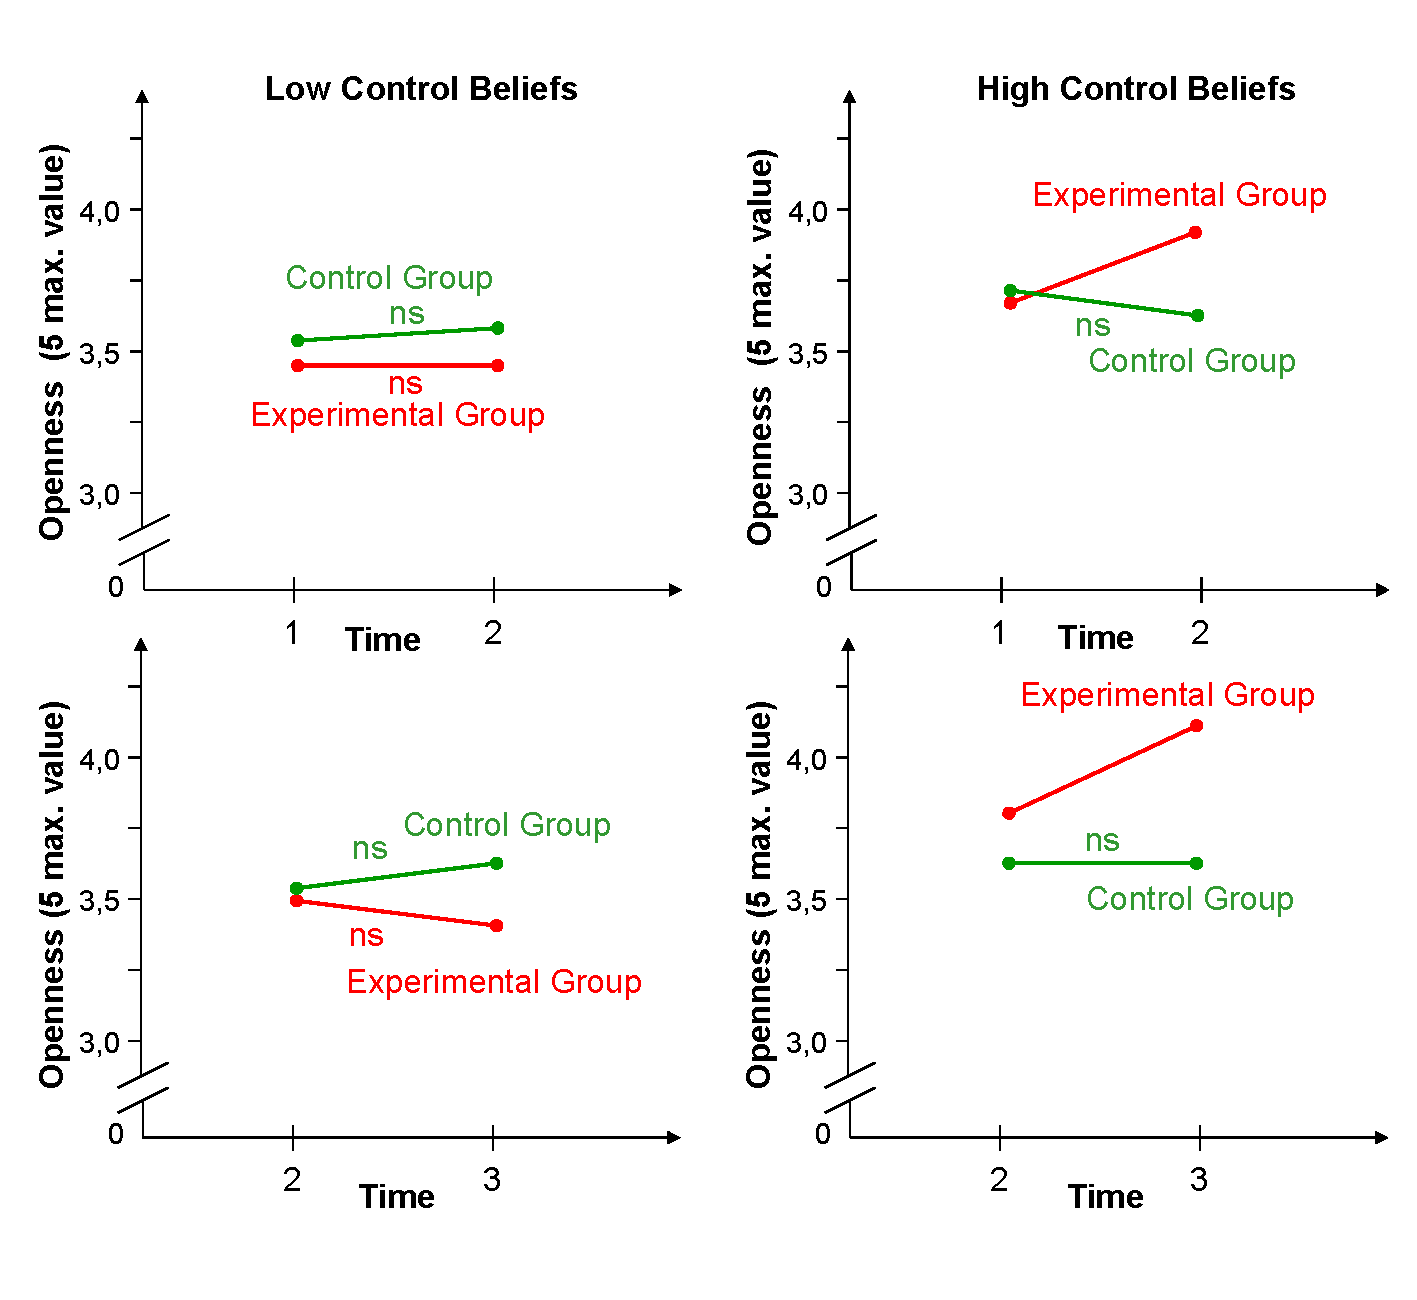
\includegraphics{profUrsulaStaudinger-fig3}}
    \caption{For participants with above median levels of internal control beliefs, the participation in the EFI program resulted in increases in Openness to Experiences. These increases were sustained across a period of 12 months (M\"uhlig-Versen \& Staudinger, in preparation).}
    \label{fig3:profUrsulaStaudinger}
  \end{center}
\end{figure}

\newpage

 All in all, the study shows that most likely it is not enough to become active to feel better but rather that specific circumstances, such as skill training and/or self-determination, need to be attended to as well.
 
\textit{The Effects of the Work Context on Adult Development}

 This is a new area of research that has started to emerge over the last year. One aspect that is of interest here is the effect of aging stereotypes present at the workplace on productivity and well being of older workers. First insights were gained from a JCLL pilot study that was conducted in the context of the Executive Master Program on Aging Workforce Management (LKI). In a sample of about 600 employees from 10 companies, we found as expected that older employees of companies with a rather negative aging stereotype showed poorer self-regulation as well as poorer job performance.


\paragraph{Collaborations}

\begin{itemize}
\item Deutsches Zentrum f\"ur Altersfragen DZA, Berlin\\ Prof. Dr. Clemens Tesch-R\"omer
\item Kassel University\\ Prof. Dr. Ekkehard Frieling 
\item Bremen University\\ Prof. Dr. Johannes Huinink
\item Yale University\\ Prof. Becca Levy, PhD
\end{itemize}

\begin{bibunit}[apalike]
\nocite{*}
\putbib[profUrsulaStaudinger3]
\end{bibunit}

\enlargethispage{2cm}
\paragraph{Grants}
\begin{itemize}
\item DFG STA 540/5 - 1/2 (PI: U.M. Staudinger): Age-heterogeneous interaction as facilitative developmental context (2003-2006).
\item BMFSFJ (PI: U.M. Staudinger): Personality development in old age: A natural intervention study (2001-2006).
\item Leopoldina (PI: U.M. Staudinger): Leotech Aging: Network that investigates Aging, Education and Work (2006-2009).
\item BMBF (PI: JCLL). U.M. Staudinger, U. Kunzmann: subproject ``Images of Aging'' within the joint research project ``Effects of Matches/Mismatches between Aspects of Human and Social Capital, Corporate Strategy and Work Organization on the Physical and Mental Well-Being of Employees''. 
\item DFG Travel Grant for Eva-Marie Kessler for Gerontological Society of America Annual Meeting 2006
\end{itemize}


\newpage
\subsection{Plasticity and Positive Development: Theoretical and
Empirical Approaches}



\index{Staudinger, M. Ursula}

\paragraph{Research Team}
Ursula M. Staudinger (Professor), Jessica D\"orner (Doctoral Fellow until 05/2006), Eva-Marie Kessler (Doctoral Fellow, graduated in January 2006; now Postdoctoral Fellow)

Human development is not determined but plastic. This is one the central contentions of lifespan psychology. Based on biological, psychological and external resources any observed development trajectory can be changed within limits. Such changes can be directed towards an improvement or a deterioration of the normally observed developmental course. It is argued that it is theoretically and empirically useful to distinguish these two kinds of plasticity. In conjunction with negative deviations from the normal developmental course the concept of resilience has been introduced into the literature. It refers to the maintenance or regaining of normal levels of functioning in the face of stressors. In contrast, positive deviations from the developmental trajectory should be subsumed under the notion of growth. When considering development as such, rather than positive or negative deviations from an expected developmental course, it again may be meaningful to differentiate between two kinds of positive developments. One is primarily geared towards the achievement of growth and the other towards adjustment. This latter distinction has been a focus of our work in 2005.

\null
\textbf{Research Highlights 2006}

Does personality stay stable after young adulthood or is there continued change throughout middle and later adulthood? For decades, this question caused heated debate. Over the last couple of years, a consensus has emerged based on recent cross-cultural as well as longitudinal evidence. This consensus confirms that indeed there is personality change in middle and later adulthood. Many authors have labeled this change personality maturation or growth. In somewhat simplified terms the observed pattern is as follows: Neuroticism declines, conscientiousness and agreeableness increase. At the same time it has been argued that this pattern of personality change is the result of coping with the developmental tasks of adulthood and thus increased adjustment. We critically examined this practice of equating developmental adjustment with growth and pointed to the necessity of defining personality growth by reference to theories of personality development as well as lifespan theory. 

\paragraph{Collaborations}

\begin{itemize}
\item Universit\"at Hildesheim\\ Prof. Dr. Werner Greve
\item University Trier\\ Prof. Dr. Sigrun-Heide Filipp
\item IUB, JCLL\\ Prof. Dr. Ute Kunzmann
\end{itemize}

\hyphenation{Ent-wick-lungs-psycho-lo-gie Hassel-horn}
\begin{bibunit}[apalike]
\nocite{*}
\putbib[profUrsulaStaudinger4]
\end{bibunit}

\newpage
\subsection{Other Professional Activities}

\begin{itemize}
\item President elect German Psychological Association (DGPs).
\item Member of the Selection Committee of the Alexander von Humboldt Foundation.
\item Member and Vice-Chairperson of the Leopoldina and acatech Committee ``Aging-Work Education''. 
\item Senior Fellow of the International Network on Aging of the Max Planck Society (MAXNETAging).
\item Member of the Scientific Board of the German Center for Gerontology (DZA) in Berlin.
\item Member of Scientific Board Center Aging \& Work (Sloane Foundation).
\end{itemize}



\textit{Editorial Board Memberships}

Psychology and Aging (since 1997), Psychologie in Erziehung und Unterricht (since 2000), Psychologie Verlagsunion Book Series ``Psychologie-Forschung-Aktuell'' (2000-2005), Book Series Psychologische Diskurse (Verlag Vandenhoeck \& Ruprecht) (since 2003), Research in Human Development (since 2003), The Journal of Positive Psychology (since 2005), Developmental Science (since 2006).




\cleardoublepage
\section{Emotional Competence and Wisdom: Lifespan Developmental Perspectives} \shorttitle{Adult Development of Socio-Emotional Competences
}

One-sided views of aging and old age still exist in our society as well as in scientific circles. On the one hand, old age has been portrayed as a period of disengagement, social isolation, cognitive inflexibility, and physical decline. On the other, many people, especially older people themselves have described old age as a productive life period full of energy, new and inspiring experiences, and gratifying moments. Lifespan developmental researchers have argued that images of old age and aging that are either too negative or too positive run the risk of being dysfunctional. Overly pessimistic views lead to disregard for the possibility that many older people have great potential and could provide valuable contributions to societal life. Illusory positive views put unnecessary pressure on those older people who have experienced age-related losses and hinder social policies aimed at improving their living situations.

 Adopting a lifespan developmental approach, the overarching goal of our research has been to contribute to a balanced picture of aging and old age that encompasses loss, continuity, and growth. According to lifespan developmental psychology, the complexity of developmental processes during adulthood can be described on at least four levels. First, development is multidirectional. During the same developmental period, some realms of functioning decline, while others remain stable, and yet others increase. Second, development is multifunctional. Depending on the criteria that are being considered (e.g., subjective vs. objective or long-term vs. short-term), the same developmental outcome can be considered as gain or loss. Third, development varies among individuals and various social, educational, and ethnic groups. Depending on the individual's personal and social resources, the same realm of functioning may decline, increase, or remain unchanged during adulthood and old age. Fourth, people do not exist in isolation, but are embedded in historical, cultural, and social contexts that provide both developmental opportunities and constraints.

 Two realms of functioning, which are at the center of our research, are ideally suited to demonstrate the complexity of the aging process on the four levels described above. These are emotional competence and wisdom. The primary purpose of our research is to demonstrate that the development of emotional competence and wisdom is differential. That is, it evinces multidirectionality, varies among individuals, is contextually-bound, and simultaneously involves gains and losses. This differentiated view of development helps expand and supplement more traditional conceptualizations that have emphasized universal and general developmental processes and equate development with growth. 

\subsection{Emotional Competence}

\index{Kunzmann, Ute}

\paragraph{Research Team}
Ute Kunzmann (Professor), David Richter (Doctoral Fellow).

 The concept of emotional competence has received widespread attention in several psychological disciplines and various definitions have recently been suggested, differing in terms of content and breadth. Ute Kunzmann and her collaborators have considered emotional competence as a multidimensional concept that covers several distinct facets, including the capacity to spontaneously react to emotion-arousing events with the appropriate emotion, the ability to voluntarily regulate one's own emotions, and the ability to accurately detect other's emotions.
 
 Keeping in mind that people's subjective evaluations of what they can do are sometimes not accurate reflections of their ``objective'' competencies, Ute Kunzmann has begun to design and conduct well-controlled experimental studies in which emotions and emotional abilities can be observed in vivo. In these studies, adults of different ages are exposed to the same emotionally challenging tasks and their subsequent cognitive and emotional reactions are observed objectively. Evidence from this research is meant to supplement the findings from studies employing self-report questionnaires and performance-based tests of emotional competence. 

Findings from the Kunzmann's and her collaborators' laboratories strongly support the general propositions of life-span developmental psychology described above. For example, there is robust evidence for multidirectionality in the realm of emotional reactivity. Whereas autonomic reactions seem to decline with age, subjective reactions remain stable. Furthermore, this pattern of age differences is not fixed but at least partly determined by contextual factors such as the age-relevance of the emotion-arousing event. When being exposed to emotion-evoking themes that are particularly salient in old age, older adult's reactions are greater or just as large than those of young adults - even on the level of autonomic activity.  

Ute Kunzmann and her collaborators at the University of California, Berkeley also provided first performance-based evidence that the ability to regulate one's own emotional reactions on command remains unchanged over adulthood and old age. This evidence refers to one particular form of emotion regulation, that is, the ability to voluntarily up- and down regulate one's facial expressions. Given that emotion regulation comprises multiple forms, the question arises of whether the current evidence can be generalized to other forms of emotion regulation (e.g., the ability to re-evaluate negative experiences so that they become less threatening to the self). An experimental study that Ute Kunzmann designed together with Prof. Fredda Blanchard Fields at the Georgia Institute of Technology, Atlanta will begin to address this question in the near future.

\null
\textbf{Research Highlights 2006}

\textit{Study on Empathic Accuracy: First Results}

 Our research activities during the last months have focused on yet another emotional ability, namely, the \textit{ability to accurately perceive other people's emotions} (i.e., empathic accuracy). As is true for so many resource-demanding and effortful functions, the empirical evidence generally suggests that young adults outperform older adults in tasks assessing this ability. However, a serious limitation of the typical paradigm used to study age differences in empathic accuracy is its lack of ecological validity. Participants are typically asked to recognize emotions from still photographs of faces, which provide very little information about the evaluated persons. Moreover, emotions are typically posed rather than truly experienced. Studying emotion recognition via tasks that are less stripped down in terms of familiarity and meaningfulness might yield a very different picture about age differences in this ability.  

 To test this proposal, Ute Kunzmann and David Richter conducted a study with more contextualized empathic accuracy tasks in our lab. Instead of presenting to young and old adults photographs of people posing prototypical emotions, they presented eight short film clips each dealing with a person as he or she was talking about an emotionally engaging issue. The to be evaluated people experienced real and authentic emotions while talking. To study the role of motivational factors, the age relevance of the topics the videotaped people were talking about was manipulated. One topic was of particular relevance to older people and dealt with age-related losses. A second topic was of particular relevance to young people and dealt with an adventurous and risky life transition. 

 As can be seen in Figure \ref{fig1:profUteKunzmann}, the age-related decline in emotion recognition found in earlier studies was only evident in situations that were of minor relevance to older people. In contrast, there was no age difference in performance level when the task was to accurately evaluate the emotions of a person who talked about a topic that was particularly relevant in old age. Two conclusions from this work are that age-related decline in resource-demanding processes may be limited to tasks and contexts that are of little relevance to older people and that motivational factors can offset age-related deficits. Ute Kunzmann and David Richter organized a symposium with the title ``lifespan development of emotions and emotional competencies'' at the 45th Congress of the German Society for Psychology in September 2006 in the context of which they presented their latest findings. In addition, they are about to submit a grant proposal to the German Research Foundation that will allow them to test additional moderators of the relationship between age and empathic accuracy.

\begin{figure}[htb]
  \begin{center}
    \resizebox{0.5\textwidth}{!}{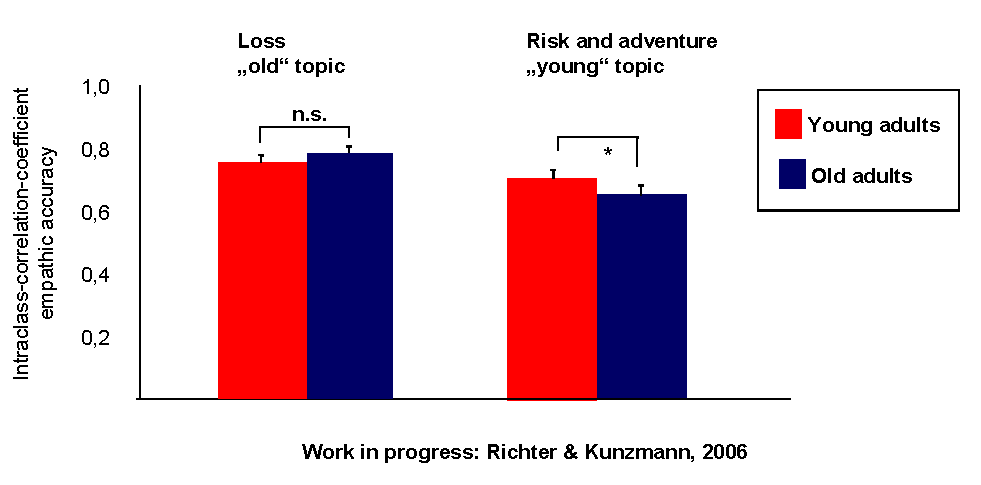
\includegraphics{profUteKunzmann-fig1}}
    \caption{Age differences in empathic accuracy: Age relevance matters.}
    \label{fig1:profUteKunzmann}
  \end{center}
\end{figure}



\textit{Research Network from the German Research Foundation}

 Another research highlight of the last year was a first meeting of a research network funded by the German Research Foundation (faculty member: Ute Kunzmann; student member: David Richter). The network consists of German researchers who study the differential and general development of emotions and emotional competencies. The network members (1/3 faculty and 2/3 graduate students) will hold two meetings per year for a period of three years. The meetings will be designed (a) to facilitate exchange of ideas and expertise, (b) to discuss research with invited internationally distinguished emotion researchers (two guests per meeting), and (c) to develop plans for future collaborative research projects.

\paragraph{Collaborations}
\begin{itemize}
\item Georgia Institute of Technology, Atlanta, USA \\ Prof. Fredda H. Blanchard-Fields, PhD
\item University of California, Berkeley, USA \\ Prof. Robert W. Levenson, PhD
\item University of Geneva, Geneva, CH \\ Prof. Gisela Labouvie-Vief, PhD
\end{itemize}

\begin{bibunit}[apalike]
\nocite{*}
\putbib[profUteKuzmann1]
\end{bibunit}



\paragraph{Grants}

\begin{itemize}
	\item BMBF (PI: JCLL). U. Kunzmann, U.M. Staudinger: subproject ``Images of Aging'' within the joint research project ``Effects of Matches/Mismatches between Aspects of Human and Social Capital, Corporate Strategy and Work Organization on the Physical and Mental Well-Being of Employees''. 
\end{itemize}



\subsection{Emotions in Art}

\index{Kuzmann, Ute}

\paragraph{Research Team}
Ute Kunzmann (Professor), Caroline Schuster Cordone (Doctoral Candidate (University of Fribourgh, Switzerland).

 This project deals with a research topic that transcends disciplinary boundaries. Funded by the International Max Planck Research Network on Aging in November 2006, the central goal of the project is to contribute to a better understanding of the ways in which emotions are expressed in paintings by joining forces and combining art historical and psychological approaches. Ute Kunzmann and her art historical colleague Caroline Schuster Cordone pan to compare art historical and psychological interpretations of the emotional expressions of young and old figures as they are depicted in paintings spanning several epochs. 

 The two psychological approaches to interpreting emotional expressions in paintings are illustrated through a self-portrait of Rembrandt in Figures \ref{fig2:profUteKunzmann} and \ref{fig3:profUteKunzmann}. As can be seen in Figure \ref{fig2:profUteKunzmann}, the expert-based approach to describing emotional expressions in paintings will be based on Paul Ekman's Facial Action Coding System. According to this system, Rembrandt expresses moderate happiness blended with another emotion, most likely slight surprise. 

\begin{figure}[htb]
  \begin{center}
    \resizebox{0.5\textwidth}{!}{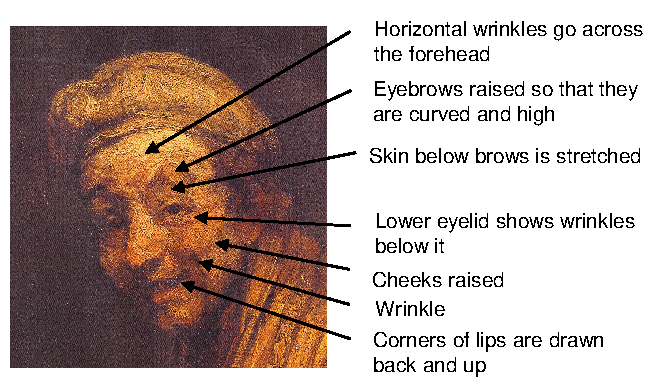
\includegraphics{profUteKunzmann-fig2}}
    \caption{Emotional expressions in paintings: An expert-based approach}
    \label{fig2:profUteKunzmann}
  \end{center}
\end{figure}

The consensus-based approach to describing emotional expressions in paintings is illustrated through the same self-portrait of Rembrandt (see Figure \ref{fig3:profUteKunzmann}). 

\begin{figure}[htb]
  \begin{center}
    \resizebox{0.4\textwidth}{!}{\includegraphics{profUteKunzmann-fig3}}
    \caption{Emotional expressions in paintings: A consensus-based approach.}
    \label{fig3:profUteKunzmann}
  \end{center}
\end{figure}

This approach is based on laypeople's intuitive understanding of emotions. In a pilot study, young and old laypeople were asked to evaluate the painting in terms of which emotions are depicted. Results supported the expert-based codings and revealed that Rembrandt expresses moderate happiness blended with slight surprise. However, there was also high consensus among laypeople that Rembrandt was mischievous and somewhat ironic. The latter two affective states are not part of Ekman's coding system.

\paragraph{Collaborations}
\begin{itemize}
\item University of Fribourg \\ Caroline Schuster Cordone
\end{itemize}

\paragraph{Grants}

\begin{itemize}
\item Maxnet Aging, Max Planck Society (Start 2007). (PI : U. Kunzmann): Expression of emotions in Art: Art Historical and Psychological Perspectives.
\end{itemize}

\subsection{Wisdom}

\index{Kuzmann, Ute}

\paragraph{Research Team}
Ute Kunzmann (Professor), David Richter (Doctoral Fellow).

 Although the psychology of wisdom is a relatively new field, several promising theoretical and operational definitions of wisdom have been developed during the last years (for reviews see Kunzmann, in press; Kunzmann \& Baltes, in press; Kunzmann \& Stange, in press). Our own work has been based on the Berlin wisdom paradigm that defines wisdom as expert knowledge about fundamental problems related to the meaning and conduct of life. In this paradigm, participants think aloud about difficult and uncertain life problems. Trained raters evaluate these think-aloud protocols according to five criteria indicating wisdom. The three core criteria are: (1) value relativism and tolerance, (2) awareness and management of uncertainty and (3) lifespan contextualism. 

 The goal of our research program has been to study the social and emotional dynamics of wisdom-related knowledge in the context of correlational field studies and experimental work. With this goal we intend to produce evidence that highlights the gains that come with the acquisition of wisdom-related knowledge during ontogenesis and especially the difference that this type of knowledge makes in adults' actual social and emotional behavior.

\null
\textbf{Research Highlights 2006}

 During the last year, Ute Kunzmann completed several publications dealing with the motivational, affective and social dynamics of wisdom-related knowledge. As to the social-emotional dynamics of wisdom-related knowledge, her experimental work suggests that people with high levels of wisdom-related knowledge tend to experience greater empathic sadness when being together with another person in need than people with low levels of wisdom-related knowledge. There is also evidence for a link between wisdom-related knowledge and empathic accuracy: wisdom-related knowledge seems to help people perceive other people's emotions accurately. 

 In her field studies Ute Kunzmann and her collaborators have demonstrated that the values and behaviors of people with high levels of wisdom-related knowledge indicate a striving for a good life in the sense of early Greek philosophy. One aspect of a good life in the early Greek tradition refers to the balancing of personal and common interests. A second aspect refers to the preference for personal growth and self-actualization -- even if this preference opposes happiness in a hedonistic and materialistic sense. Together the evidence from Ute Kunzmann and her collaborators strongly supports the general hypothesis that wisdom-related knowledge makes a difference in people's daily life and has important motivational and social functions for one's own and others' development. 

\newpage
\paragraph{Collaborations}
\begin{itemize}
\item Georgia Institute of Technology, Atlanta, USA  \\ Dr. Antje Stange
\item Tufts University, Medford, USA \\ Prof. Robert J. Sternberg, PhD
\end{itemize}

\enlargethispage*{0.2cm}

\begin{bibunit}[apalike]
\nocite{*}
\putbib[profUteKunzmann3]
\end{bibunit}

\subsection{Awards, Fellowships}
\begin{itemize}
\item Junior Fellow of the Max Planck International Research Network on Aging. 
\end{itemize}

\subsection{Other Professional Activities}  

\begin{itemize}
\item Consultant on methods to assess physiological and behavioral aspects of emotion with NIH Project; PI: Prof. Dr. Blanchard-Fields, Georgia Institute of Technology, Atlanta.
\item Faculty member of the research network ``Differential and General Development of Emotion'' funded by the German Research Foundation (HO 1718/5-1).
\end{itemize}

\textit{Editorial Board Membership}

\begin{itemize}
\item Psychology and Aging.
\end{itemize}

\vspace{0.5ex}
\textit{Ad-hoc Reviews}

\begin{itemize}
\item Swiss National Science Foundation.
\end{itemize} 


\cleardoublepage
\section{The Communication of Information and Knowledge: An
Important Facet of Lifelong Learning} \shorttitle{Communication of Information and Knowledge}

Media are (external) information storage devices and transmitters. Knowledge is the internal representation of information including the relations of all the components in a living being. Lifelong learning means acquiring knowledge at all stages of life. Three different kinds of knowledge - among others - can be identified: 
\begin{itemize}
	\item Procedural knowledge (e.g., setting the VCR-timer).
	\item Social and semantic knowledge (e.g., Alois Alzheimer was born in 1864). 
	\item Personal knowledge (e.g., what wartime was like).
\end{itemize}

The human species is the only species that can transfer knowledge by an elaborate system of communication. Humans learn throughout all their life, they are able to plan ahead by imagining, rehearsing and evaluating situations. Humans can do that mentally, in games and by watching or listening to others - even by reading a book, surfing the internet, listening to radio or watching TV or a movie. 

 Our overarching research question is what roles media play for lifelong learning and if age differences can be identified.

\subsection{BALANCE: The Effects of Media Communication}

\index{Schwender, Clemens}

\paragraph{Research Team}
Clemens Schwender (Professor), Siegmar Otto (Doctoral Fellow), Dennis Mocigemba (Postdoctoral Fellow), Aynur Huylu (Dipl. Media Consultant), Claudia Hesping (Dipl. Media Consultant), Hatice Ecirli (Student Assistant), Florin Bora (Student Assistant)

 Project BALANCE: Why do people turn off the TV? This is the question that the BALANCE project tries to answer with regard to sustainability communication on TV. Sustainability communication faces the criticism that it reaches only those, who are informed anyway, and that a great part of society is not reached at all. Viewers turn off, or switch between channels and thereby refuse reception. The BALANCE project tries to change that by developing and implementing the concept of ecotainment: Messages about sustainability are to be combined with positive emotions.

 By applying content analysis (to identify narrative structure, offered messages and symbols for ecology and sustainability) as well as on- and offline questionnaires (to identify emotional impact, memory and attitudes toward the presented messages), we develop concepts for educational materials and inform journalists and production teams about our findings. The ultimate goal of the project is to broaden knowledge about sustainability in the population.

\null
\textbf{Research Highlights 2006}

\textit{The Avoidance of Information}

 When people watch TV, they use the remote control to decide about the information they will accept. So far, research on strategies of switching channels was centered mainly on the context of commercial avoidance. In my working group, we have developed a model that is able to determine reasons for switching channels that captures not only the content level, but also other factors, such as film aesthetics. The goal is to develop different categories to improve knowledge transfer, especially within the informal context of mass communication.

 Since Fall 2006 we finally have access to media ratings on a second-by-second basis. Now we will be able to find the moments (and reasons) when (and why) people switch channels while watching reports that contain knowledge information. The reasons can be clustered in three domains: (a) Context (like position of the episode, the position in relation to commercial breaks, the program of competitive channels), (b) Content (like interview situations, the presentation of big machines and production lines, the three dimensions - social, ecological and economical - of sustainability), and (c) Formal Aspects (like duration, number of cuts per minute). Our preliminary results indicate that an episode is accepted when it fits the viewers expectations in respect to the program. In the context of ``Welt der Wunder'' sustainability is an accepted topic. 

\textit{Investigation of Media Strategies for Audio-Visual Arguments}

 My working group is also investigating a representative sample of TV-Commercials to better understand what strategies media use for making audio-visual arguments. The term ``narrative function'' is able to explain how characters are used. For the first time, the categories age and gender are not used in content analysis to determine the respective demographic representation, but to determine their function as a stereotypical argument. The goal is to learn how commercials succeed in making a convincing audio-visual argument in a very short time.

 The content analysis of 698 TV-spots for products and services but also for social behavior or awareness and for political parties is finished. The spots present more than 5.000 agents.

\textit{Investigation of the Public Debate on Sustainability in TV and Print Media}

 With the support of ``google news'' we are able to check 700 papers daily for the terms ``sustainability'' and ``sustainable development''. Long-term studies were made with the daily paper ``Die Tageszeitung'' and the weeky paper ``Die Zeit'' from 2002 to 2005. The data show that great events like the Johannesburg World summit in 2002 had a verifiable impact on the coverage of sustainable development in Germany.

 Twice a year, we look at a TV Guide to detect all possible shows that may include issues that deal with sustainability. The media survey suggests a bigger potential for public debate on sustainability.

\newpage
\textit{Transfer of results}

 We are currently preparing a series of workshops for journalists as well as for experts in the field of sustainability research. The workshops will be organized by the Adolf-Grimme-Institut (Marl) and the Bundespressekonferenz (Berlin). 


\paragraph{Collaborations}
\begin{itemize}
\item Universit\"at Hohenheim \\ Lehrstuhl Umweltmanagement \\ Prof. Dr. Werner F. Schulz; Martin Kreeb; Volker Diffenhard 
\item Copenhagen Business School \\ nwd Institut \\ Dr. Lucia Reisch 
\item .lichtl Sustainability Communications \\ Martin Lichtl
\item Adolf-Grimme-Institut, Marl \\ Dr. Friedrich Hagedorn 
\end{itemize}

\begin{bibunit}[apalike]
\nocite{*}
\putbib[profClemensSchwender]
\end{bibunit}

\paragraph{Grants}

\begin{itemize}
\item BMBF (PI: C. Schwender). B.A.L.A.N.C.E. Development, Application and Promotion of a Communicational and Trendsetting Concept for a Sustainable Life and Management 2004-2006.
\end{itemize}

\newpage
\subsection{Technical Documentation: Age-related Formatting of Information}

\index{Schwender, Clemens}

\paragraph{Research Team}
Clemens Schwender (Professor), Christoph K\"{o}hler (Dipl. Media Consultant), Ulrich B\"{u}hring (Student Assistant Donau University Krems).

 In our homes and at work we are confronted with new technology. Written, AV- or online-documentations explain how to build or handle these artefacts. Again and again we are faced with situations in which technology is not self-explaining but needs introduction instead. Media-based teaching happens without the presence of a teacher. People must read and understand text and pictures. Formatting and design play crucial roles in the motivation to access user's manuals. There is no option of asking questions and receiving immediate answers. Manuals must reflect the restrictions and preferences of the users of different age, gender and cultural background.

\begin{figure}[h]
  \begin{center}
    \begin{minipage}[b]{0.35\linewidth}
   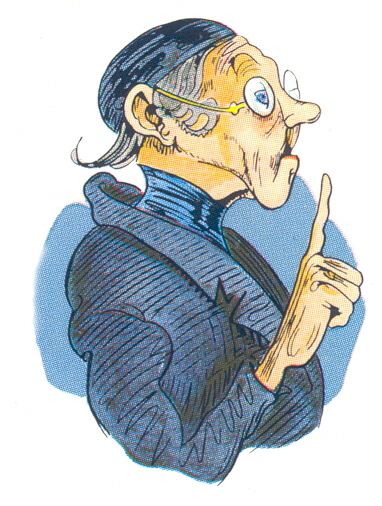
\includegraphics[width=\linewidth]{profClemensSchwender-fig1.jpg}
    \end{minipage}\hfill
    \begin{minipage}[b]{0.55\linewidth}
      \caption{Taken from Wilhelm Busch (1865): Max und Moritz. This kind of humorous dispersal is not accepted in technical documentation.\label{fig1:profClemensSchwender}}
    \end{minipage}
  \end{center}
\end{figure}

 Technical documentation is usually associated with boring reading. People avoid taking the manuals in their hands. We are investigating how motivation can be improved by making changes in the design: The page layout, font type and font size are considered as well as the use of more pictures and pictures that portrait not only machines but also people. The role of humor will be tested, to see if it has an influence on the motivation to look at a manual and to read it.

\null
\textbf{Research Highlights 2006}

 The research on technical documentation is a prototype for learning in adulthood. Technical documentation is an important example of lifelong learning. We try to observe how the learning process takes place without the presence of a teacher. In our working group we look at the formatting of information and test different conditions with persons of different age. 

 First results indicate that color and font size play a positive role and can be considered as motivational factors. Humor and comic-style pictures provoke resistance against the documentation. Effects on the speed of transforming reading into action and the accuracy of accomplishment cannot be found.


\paragraph{Collaborations}
\begin{itemize}
\item tekom - Der deutsche Fachverband f\"{u}r Technische Kommunikation und Informationsentwicklung
\end{itemize}

\begin{bibunit}[apalike]
\nocite{*}
\putbib[profClemensSchwender2]
\end{bibunit}

\subsection{Feldpost-Archiv} 

\index{Schwender, Clemens}

\paragraph{Research Team}
Clemens Schwender (Professor), Thomas Jander (Student Assistant, Humbold University Berlin), Dr. Jens Ebert (Literature Historian), Elena Nedbaylo (PhD Candidate), Dr. Ortwin Buchbender (Military Historian)

 The Feldpost-Archiv is an archive for the war time generation's personal knowledge. Media are used to communicate experience, opinions, and knowledge. E-mails, letters, and the telephone are examples of individual media. The problem of investigating their content and usage is that they are usually not stored, but forgotten, deleted or thrown away - with one unique exception: Feldpost letters. With the Feldpost Collection, Feldpost letters will be catalogued and coded for scientific use. The data will be accessible over the Internet. The goal is to build a representative, web-based collection of war letters.

 Personal memories, experiences and written statements of the war generation are a valuable subject for research on memory and media, as well as for political psychology. Based on such collections, for instance, background questions about the age-graded effects of propaganda can be asked and hopefully answered in the near future. 

\begin{figure}[h]
  \begin{center}
    \begin{minipage}[b]{0.40\linewidth}
   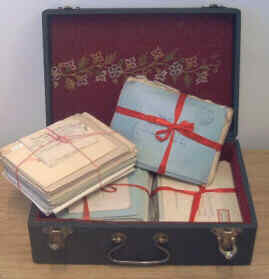
\includegraphics[width=\linewidth]{profClemensSchwender-fig2.jpg}
    \end{minipage}\hfill
    \begin{minipage}[b]{0.55\linewidth}
      \caption{Collection of letters in the Feldpost-Archiv in Berlin, initiated by Clemens Schwender.\label{fig2:profClemensSchwender}}
    \end{minipage}
  \end{center}
\end{figure}

\textbf{Research Highlights 2006}

 This year our work concentrated on a survey of so called ``gray literature''. These are publications and editions of war letters and memoirs by war participants or their relatives. Usually these are not critical editions and lack information on provenance. But nevertheless they are important for war letter research and provide a useful source of information if handled with care.

%\begin{figure}[ht]
%  \begin{center}
%    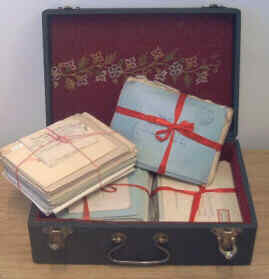
\includegraphics[width=7.5cm]{profClemensSchwender-fig2.jpg}
%    \caption{Collection of letters in the Feldpost-Archiv in Berlin, initiated by Clemens Schwender.}\label{fig2:profClemensSchwender}
%   \end{center}
%\end{figure}

\paragraph{Collaborations}
\begin{itemize}
\item Museum of Communication Berlin \\ Prof. Dr. Joachim Kallinich
\item State Library Stuttgart \\ Prof. Dr. Gerhard Hirschfeld
\item Prussian Cultural Heritage in Berlin, State Library \\ Dr. Jutta Weber 
\item University of Witten/Herdecke \\ Prof. Dr. Harald Welzer
\item State University Surgut, Russia \\ Dr. Vasiliy Glushak
\end{itemize}

\begin{bibunit}[apalike]
\nocite{*}
\putbib[profClemensSchwender3]
\end{bibunit}

\subsection{\mbox{Age, Emotions and Media-Preferences}}

\index{Schwender, Clemens}

\paragraph{Research Team}
Clemens Schwender (Professor).

 People choose what papers they buy, what they read, to what TV-channels they switch, what movies they like and which ones they want to see. This changes during the course of life, but so far no detailed research has been done on this topic.

 Basic answers are still needed: 
\begin{itemize}
	\item Why do people cry, get scared or laugh during movies or while reading a novel?
	\item How and why do preferences change?
	\item Can that be explained by age factors?
\end{itemize}

\null
\textbf{Research Highlights 2006}

 A survey about the reasons why older adults don't go to the movie theaters anymore contained the question about the personal favorite movie. The answers to this particular question raised our interest and led to a broader research question about age-related media- and genre-preferences. The most mentioned movie in the age groups of persons older than 49 is ``Gone with the Wind''.  A wider survey is being conducted. Besides the preferences and the reasons for their selection, there are also items to identify the reception modalities as developed by Monika Suckf\"{u}ll.

%\begin{figure}[ht]
%  \begin{center}
%    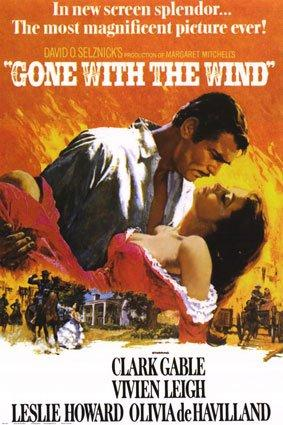
\includegraphics[width=7.5cm]{profClemensSchwender-fig3.jpg}
%    \caption{Most Germans (50+) claim "Gone with the Wind" to be the best movie of all times.}\label{fig3:profClemensSchwender}
%   \end{center}
%\end{figure} 

\begin{figure}
  \begin{center}
    \begin{minipage}[b]{0.40\linewidth}
   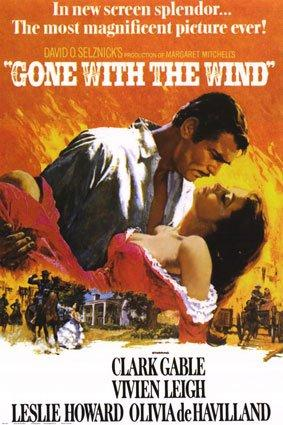
\includegraphics[width=\linewidth]{profClemensSchwender-fig3.jpg}
    \end{minipage}\hfill
    \begin{minipage}[b]{0.55\linewidth}
      \caption{Most Germans (50+) claim "Gone with the Wind" to be the best movie of all times.\label{fig3:profClemensSchwender}}
    \end{minipage}
  \end{center}
\end{figure}


 Preliminary results show that genre preferences change during the lifespan. Preferences change according to age/cohort. Older people favor less aggressive genres like Western, Sciences Fiction or adventure movies. Older people also prefer movies that deal with time periods that they know from their own past experience: Movies about the time and events of World War II are often preferred to movies about contemporary issues. In this category you can find movies like ``The Downfall'' or ``The Boat''. Persons over 70 never mention movies about the future (Science Fiction) as their favorites.

\paragraph{Collaborations}
\begin{itemize}
\item Hochschule f\"{u}r Film \& Fernsehen, Potsdam \\ Dr. Dagmar Hoffmann
\item Universit\"{a}t der K\"{u}nste, Berlin \\ Prof. Dr. Monika Suckf\"{u}ll 
\end{itemize}

\begin{bibunit}[apalike]
\nocite{*}
\putbib[profClemensSchwender4]
\end{bibunit}


\subsection{Identification of Matches and Mismatches in Communication at the Work Place}

\index{Schwender, Clemens}

\paragraph{Research Team}
Clemens Schwender (Professor), Sven Voelpel (Professor)

 Communication is a central part of a company's wealth. Also communication can be a cause for getting sick. We need to identify the factors that support healthy communication styles and how individuals, leadership, and the overall climate can support healthy communication. The balance between asking for and providing information must be identified.
 
\paragraph{Grants}
\begin{itemize}
\item BMBF (PI: JCLL). C. Schwender, S. Voelpel: subproject ``Communication and Experience Management'' within the joint research project ``Effects of Matches/Mismatches between Aspects of Human and Social Capital, Corporate Strategy and Work Organization on the Physical and Mental Well-Being of Employees''.  
\end{itemize}

\enlargethispage{2cm}
\subsection{Other Professional Activities}

\begin{itemize}
\item Reviewer for ICA-Conference in San Fransisco 2007.
\item Reviewer for DGPuK-Conference in Bamberg 2007.	
\end{itemize}


\cleardoublepage
\section{A Lifespan Perspective on Organizational Behavior}
\shorttitle{A Lifespan Perspective on Organizational Behavior}

Organizational behavior research addresses the interplay of organizational context - expressed in an organization's culture, climates and goals - and organization members' KSAOs - the I/O Psychology shorthand for knowledge, skills, abilities and other characteristics (e.g., motives, personality, values). Until recently, age-related KSAO changes have not been much of a concern. The business place has been - and still is - youth-centered, and research projects have reflected this. In the wake of demographic change, however, a growing number of older (50+ yrs) workers will live longer work lives. At the same time, fewer younger workers will be available. As globalization and technological change pace permanent adaptation, continuous learning will become an integral part of organizations' operating systems. 

 On this background, an important overarching question will be how the developments of an organization and of its members may best be aligned for the benefit of both sides. More specifically, a fruitful research agendum will be to apply concepts and findings from lifespan psychology to develop an age-differentiated theory that describes how organizational and individual learning needs and abilities can best be matched. With a view on individuals, this will require to uncover the system of age-related changes in workplace behaviors. With a view on companies, it will be necessary to develop competency management approaches that take the dynamics of individual development into account.

\subsection{Successful Workplace Learning across the Lifespan}


\index{Ro\ss nagel, Christian}

\paragraph{Research Team}
Christian Ro\ss nagel (Professor, since 09/2006), Melanie Schulz (Doctoral Fellow, starting February 2007).

\enlargethispage{0.5cm}
 This research line aims at describing age-related changes in individual workplace learning. Our basic assumption is that organizational and personal factors will interact so that age will moderate the influence of organizational factors on the perceived learning context (personal-subjective factors), and thus lead to different learning success. Subjective factors are assumed to be more important to learning success than objective factors. Clarifying the regularities of the interplay between organizational and personal factors will broaden our understanding of adult development at the workplace, and help develop and extend age-adequate HRD practices. Learning success is generically defined as the maximization of desired learning outcomes and minimization of undesired learning outcomes.

 As a first empirical step, we will develop age-differentiated instruments to assess motivational and affective consequences of learning episodes, and the learning climate of organizations. These questionnaires will be drafted from literature reviews, similar instruments and calibrated in semi-structured interviews. Construct validity will be assessed in a web-based survey. The survey will address participants who have recently participated in Training and Development measures. In a second step, we will experimentally validate the assumptions of the theory to be developed by investigating the interplay of age and \textit{developmental interactions} at the workplace. The experiments will test for the impact of different adviser styles on advisees' learning success. The topic of advice will be a computer task that will be novel to participants, but related to their everyday work, and likely to be used both by younger and older participants.

\paragraph{Collaborations}
\begin{itemize}
\item University of Heidelberg, Psychology Dept \\ I/O Psychology Unit \\ Prof. Dr. Guido Hertel; Dr. Ralf Stegmaier
\end{itemize}

\enlargethispage{0.5cm}
\begin{bibunit}[apalike]
\nocite{*}
\putbib[profChristianRossnagel]
\end{bibunit}

\paragraph{Grants}

\begin{itemize}
\item BMBF (PI: JCLL). C. Ro\ss nagel, K. Sch\"omann: subproject ``Learning'' within the joint research project ``Effects of Matches/Mismatches between Aspects of Human and Social Capital, Corporate Strategy and Work Organization on the Physical and Mental Well-Being of Employees''. 
\item DFG (submitted, PI: C. Ro\ss nagel with U.M. Staudinger in the framework of the DFG focus program 1293). Age-differentiated analysis of the competency of self-regulated professional learning.
\end{itemize}


\subsection{Dynamic Modeling of Lifelong Learning Competency}

\enlargethispage*{1cm}

\index{Ro\ss nagel, Christian}

\paragraph{Research Team}
Christian Ro\ss nagel (Professor, since 09/2006), Michael Kohler (Diploma Student).

 Competency models are widely used by Human Resource (HR) practitioners in the selection, placement and development of employees. However, only little competency modeling research has been conducted, and the issue of age-related competency changes has hardly ever been addressed. In collaboration with Bosch Rexroth AG, we are developing a competency model that incorporates employees' age-related changes in ability and motivation factors. The model is intended to help identify HR development requirements in the mid-term (5 years).

 Using a goodness-of-fit framework, we will match supervisors' ratings of their employees on competencies described in existing company-specific competency models against employees' ratings of their KSAOs and their perception of how these will change over the next five years. Fit indices will be computed for ability and non-ability-related dimensions to identify mismatches as a starting point for HR development measures.

\textbf{Collaborations}
\begin{itemize}
\item Bosch Rexroth AG, Homburg Plant \\ Personnel Department \\ Claudia Neunzig
\end{itemize}


\subsection{Organizational Determinants of Vocational Adjustment Disorders}


\index{Ro\ss nagel, Christian}

\paragraph{Research Team}
Christian Ro\ss nagel (Professor, since 09/2006), Philipp Martzog (Doctoral Student).

 This line of research complements the research outlined in Section 9.1 that uses the concept of \textit{successful} workplace learning. Learning success will be defined not only with regards to its objective learning outcomes, but also with respect to the psychic costs it incurs. Initial informal surveys in a co-operating clinic (see 9.3.2) showed that the need for lifelong learning may turn to ``learning pressure'' and lead to severe health problems.

 We are planning to use the instruments developed in the workplace learning research (see Section 9.1) together with semi-structured interviews with patients to uncover the joint contribution of age differences and organizational factors to vocational adjustment disorders. These findings will broaden our understanding of successful workplace learning and will contribute to development of HR development and intervention strategies.

\paragraph{Collaborations}
\begin{itemize}
\item Baar Clinic for Behavioral Medicine, Donaueschingen \\ Bernd Haves (Medical Director)
\end{itemize}


\subsection{Other Professional Activities}

\textit{Editorial Board Membership}

\begin{itemize}
\item Journal of Behavioural Sciences.
\end{itemize}

\textit{Ad-hoc Reviews}

\begin{itemize}
\item Journal of Behavioural Sciences.
\item Swiss National Fund.
\item Zeitschrift f\"ur Personalpsychologie.
\item Zeitschrift f\"ur Sozialpsychologie.
\end{itemize}






\cleardoublepage
\section{A Perspective from Business Administration on the Aging Workforce} \shorttitle{Business Administration and the Aging Workforce}

\textit{``Where is the Wisdom that is lost in Knowledge, Where is the Knowledge lost in Information?''} \\- T.S. Elliot
 
 For demographic fitness, organizations, and in particular companies, need to deal first with an aging workforce and second with achieving global competitiveness through outsourcing, currently focusing on Asia as region with the largest economic growth. 

 For WISE Organizations four key levers can be identified: 

\begin{center} \textbf{Wisdom   Innovation   Strategy   Energy} \end{center}

 Therefore, the JCLL Business Administration area named WISE research group focuses on these four levers with WISE in general as well as WISE Aging and WISE Asia (see Figure \ref{fig1:profSvenVoelpel}).

 Valuable solutions for managing lifelong learning and institutional development need to combine both profound research on and investigation into key levers that determine organizational success.

\begin{figure}[htb]
  \begin{center}
    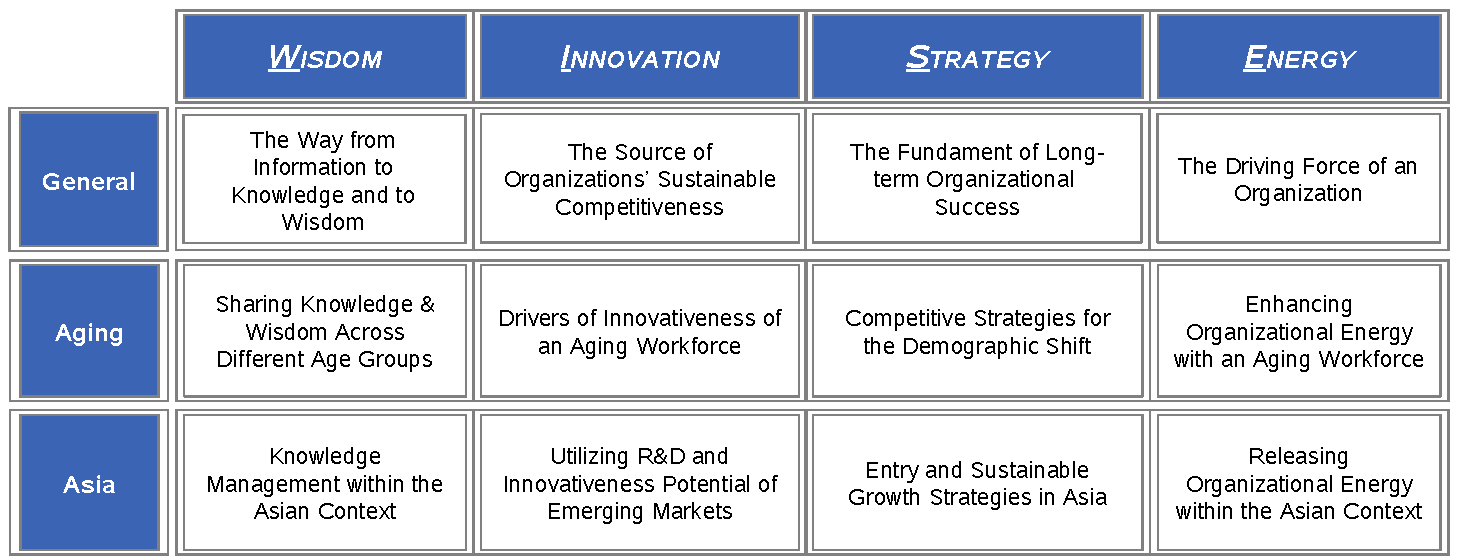
\includegraphics[width=0.5\textwidth,height=5cm]{profSvenVoelpel-fig1}
    \caption{Illustration of the different research areas of the WISE research group.}
    \label{fig1:profSvenVoelpel}
  \end{center}
\end{figure}

\newpage
\subsection{Wisdom}



\index{Voelpel, Sven}

\paragraph{Research Team}
Sven Voelpel (Professor), Zheng Han (Postdoctoral Fellow until 09/2006), Chris Streb (Doctoral Fellow), Jan Meyer (Doctoral Fellow), Chunli Zhao (Doctoral Fellow).

 Wisdom creation research has been developed from well-known streams of management research, such as information and knowledge management. Knowledge accordingly is considered as companies' basic ``resource''. Since organizations are not only driven by intellects, but also by humans, successful management research and practice also need to include less concrete constructs, such as emotional qualities. One aspect of these wisdom-related qualities would be the ability to abstract from experience knowledge and apply it to new situations.

 Research in psychology shows that wisdom is a phenomenon that depends on the successful integration of mind and character (Baltes \& Staudinger, 2000). This can be applied beyond the individual to the group and organizational level in order to create and sustain a wise organization.

 Research in the area of wisdom involves projects on: (1) knowledge management and mobilization, (2) lifelong learning, (3) knowledge acquisition for leaving/retiring employees and (4) the ``wisdom creating company''.

 With mass retirement of mature and skilled aged professionals, organizations forfeit their chances to profit from and utilize a huge pool of valuable experience, which has been accumulated by seniors during their long working career. It is becoming clear that companies risk losing wisdom and with it competitive advantage, if they let their mature workforce depart. In the light of growing organizational interest in how best to manage mature employees with rich accumulated wisdom, the paucity of research in this area represents a serious gap in academic knowledge.

 Research in the area of wisdom and aging focuses especially on: (1) knowledge management: Driving knowledge sharing and creation by supporting the natural (often social) knowledge processes with organizational and IT tools; (2) managing a multi-generational workforce: integration, participation and collaboration; (3) lifelong learning with an aging workforce; (4) knowledge acquisition for retiring employees. 

 It is a long journey starting from pure Information to Knowledge to finally reach Wisdom. The management of knowledge makes up the principal portion of this journey. Within the Asian context, Knowledge Management (KM), a well-established management research concept in the West, has been introduced not long ago. The context, however, is a totally different one due to significant discrepancies between Asian and Western cultures. Culture shapes assumptions about what knowledge is, defines the relationship between individual and organizational knowledge, creates the context for social interaction in which knowledge will be used, and shapes the processes by which new knowledge is created, leveraged and distributed in organizations. Consequently, it is of high significance to build up effective KM strategies within the Asian context.

 Research in the area of Wisdom and Asian focuses on: (1) knowledge creation in the Asian context, (2) cultural influences on the behavior of knowledge sharing, (3) best practices of knowledge management in China, (4) applicability of Western knowledge management tools within the Asian context.

\null
\textbf{Research Highlights 2006}

 In order to be able to fuse the latest streams of research in the area of knowledge management and wisdom, the research group made an effort to review the latest findings, which resulted in a number of publications (see below). Particularly noteworthy is the special issue ``Becoming critical on Intellectual Capital'' in the Journal of Intellectual Capital co-edited by David O'Donnell, Lars Bo Henriksen and Sven Voelpel. This special issue achieved to review contributions from the leading authors in the field of intellectual capital. Another extraordinary achievement is the review article on the progress in the major management field knowledge management during the last 15 years in collaboration with two of the leading researchers of the field (Nonaka, I., von Krogh, G., and Voelpel, S., 2006).

 Following efforts from last year, the group contributed to the field of Intellectual capital (IC), which is concerned with the valuation and management of intangibles such as knowledge, human capital and brands. Drawing on Habermas' theory of communicative action and an illustrative series of interviews at Meyer Werft, O'Donnell et al. (2006) describe how large parts of organizational knowledge are tacit, thus tied to individuals, yet collectively created and maintained by communicative action. This tacit background knowledge is an important driver for individual action (e.g. when professional pride motivates innovative behavior) and thus opens up promising venues for indirect (``second-order'') management of these motivators.  As central argument the authors show limits in accessing the background knowledge stemming from its truly tacit nature and thus also imposing limits on valuing the full spectrum of organizational knowledge for the purpose of cost accounting and financial reporting. Jan Meyer presented the paper at the 2nd Workshop on Visualizing, Measuring and Managing Intangibles and Intellectual Capital, Maastricht (NL).

 As preparation for further data acquisition, a survey was worked out, which links different activities (routine tasks, innovation related tasks, problem solving efforts etc.) to knowledge types and knowledge tools use from the perspective of individual employees. Here ``knowledge tools'' include not only IT-tools but also human centered tools such as meetings and master/apprentice co-working arrangements. The aim is to understand tool usage patterns as basis for optimizing the use of knowledge tools within organizations. The pilot study for next year's survey is currently conducted at Meyer Werft.

\newpage
\paragraph{Collaborations}
\begin{itemize}
\item Intellectual Capital Institute of Ireland  \\ David O'Donnell 
\item Harvard Business School, USA \\  Dorothy Leonard
\item Hitotsubashi University, Japan \\ Prof. Ikujiro Nonaka
\item Babson College, USA \\  Prof. Thomas H. Davenport, PhD
\item University of St. Gallen, Switzerland \\  Prof. Dr. Georg von Krogh
\item University of Stellenbosch, South Africa \\  Prof. Dr. Marius Leibold
\item IUB, JCLL \\  Prof. Dr. Christian Ro\ss nagel
\end{itemize}

\begin{bibunit}[apalike]
\nocite{*}
\putbib[profSvenVoelpel1]
\end{bibunit}


\paragraph{Grants}

\begin{itemize}
\item BMBF (PI: JCLL). S. Voelpel, C. Schwender: subproject ``Communication and Experience Management'' within the joint research project ``Effects of Matches/Mismatches between Aspects of Human and Social Capital, Corporate Strategy and Work Organization on the Physical and Mental Well-Being of Employees''. 
\item DAAD ``STIBET-Doktorandenf\"orderung'' PhD Seminar (Sven Voelpel, Zheng Han). 
\item Meyer Werft (Funding for PhD Thesis of Jan Meyer).
\item Stiftung der Deutschen Wirtschaft (sdw) Scholarship (Chunli Zhao). 
\item DFG Travel Grant for Sven Voelpel for Academy of Management Conference 2006, European Academy of Management Conference 2006.
\item DFG Travel Grant for Zheng Han, IAMOT Conference 2006.
\item Advanced Institute of Management Travel Grant for Sven Voelpel and Zheng Han for Workshop on the Practice of Dynamic Capabilities.
\item Singapore Management University Travel Grant for Sven Voelpel and Zhang Han for the 3rd International Research Conference on Chinese Entrepreneurship and Asian Business Networks.
\end{itemize}





\newpage
\subsection{Innovation}

\index{Name, First Name}

\paragraph{Research Team}
Sven Voelpel (Professor), Zheng Han (Postdoctoral Fellow), Chris Streb (Doctoral Fellow), Jan Meyer (Doctoral Fellow), Chunli Zhao (Doctoral Fellow).

 Innovation is currently regarded as a key factor for organizational success. This is supported by research indicating that innovative products create 80\% of companies' future revenues. Organizations aiming to survive and succeed in the highly competitive global innovation economy urgently need to adapt and innovate (reinvent) their organizational structure, business model and culture. They have to manage and enhance their innovation capabilities to create and sustain a wise organization. Research into innovation entails projects on: organizational adaptability and (disruptive) innovation, business model reinvention.

 High innovativeness has become the most important competitive edge of technology intensive firms, especially in developed economies. However, many developed economies, such as Germany, are facing a challenging phenomenon, i.e. a rapidly aging workforce. The critical question that arises is to what extent an aging of its workforce affects the innovativeness of a company and therefore their competitive advantage? Organizations that aim to sustain the pace of continuous innovations in a technology-intensive era urgently need to understand what threats and challenges are brought to them by significant demographic changes.

 Research in the area of innovation and aging focuses especially on: Aging workforce impact on innovation, enhancing innovation with an aging workforce, managing an aging workforce to sustain continuous innovations, age-heterogeneous work groups for enhanced innovation. 

 Until now, multinational companies (MNCs) in emerging markets of Asia, such as China, have mainly been concentrating on production-oriented investments. Due to an ongoing extension of competition, low cost production alone will likely fail to help firms to stay competitive in the long run. Differentiation through innovation will become a new and strategic move for many MNCs' operation in Asia. To succeed in this endeavor they need to realistically evaluate the major benefits and challenges and understand how innovations can be generated and R\&D activities can be managed under entirely different circumstances. This entails that local R\&D and innovation activities are also integrated into the MNC's global network.

 Research consequently focuses on benefits and challenges of building R\&D activities in emerging markets such as China and India, management of intellectual property, cooperation management, integration of local R\&D activity into the global R\&D network.

\null
\textbf{Research Highlights 2006}

 Further developing and deepening the innovation stream of research a number of articles have been published last year in collaboration with our collaborators, the prominent researchers in the field such as Professors Leibold and Davenport. The articles aim to bridge the innovation topic with important organizational issues such as leadership and strategic management.

 In a pursuit to tackle an impact of the aging workforce on the innovation process, our research group in collaboration with a new research partner Professor Van Der Vegt has designed a research project proposal ``The Effects of the Aging Workforce on the Innovation Process: A Large-Scale Study of Technology Intensive Companies''. Although research into the aging workforce is beginning to gain momentum, a conceptual framework that explains impacts of the aging workforce on the innovation process is nonexistent. This research product is expected to make an important contribution to academic research by explicitly addressing this issue. In this project, our research group aims to combine insights from organizational demography, innovation and organizational psychology research, to develop and test hypotheses that explain differences in innovative work behaviors across age cohorts at different activity levels. Knowledge of the differences in idea generation patterns, innovation promotion and implementation work behaviors across age cohorts will enable organizations to leverage the unique expertise and skills of their age diverse workforce. The project proposal is under review at one of Germany's major foundations. 

 The project proposal has been presented by Sven Voelpel and Polina Isichenko at the 66th Annual Academy of Management Meeting, August 2006, Atlanta, USA on ``Managing the Aging Workforce - Leadership towards a new Weltanschauung'' workshop organized by the track convenors Sven Voelpel and Chris Streb. The participants of the workshop and scholars that provided feedback included new academic collaborators of our research group were Professors David DeLong and Barbara Lawrence. 

 As a first stage of the project, interview guidelines and a survey were worked out, linking age with types of innovation, innovative activities, innovative factors and motivation. According to the preliminary agreement with Meyer Werft, the first application of this survey is currently in the pilot phase and will be tested at the company in the beginning of 2007.

 A new six months research and consulting project on innovation has been set up by Zheng Han and Sven Voelpel with five companies, i.e. Astrium Space Transportation, KAEFER Isoliertechnik, Meyer Werft, OHB Systems and Rheinmetall Defence Electronics. Aim of the project headed by Zheng Han will be to release innovation potentials of organizations. By working together with these innovation-oriented companies, the project will tackle questions such as, How to systematically identify new areas and ideas of innovation? Which kind of organizational design supports innovation? How to effectively invest and distribute corporate resources for innovation? How to create innovation through cooperation with customers, suppliers and other third parties? The kick-off event of this project was in December 2006. 

\newpage
\paragraph{Collaborations}
\begin{itemize}
\item  Harvard University \\ Technology and Operations Management \\ Prof. Alan MacCormack, PhD
\item  Harvard Business School, USA \\ Dorothy Leonard
\item  Tsinghua University, China \\ Prof. Dr. Max von Zedtwitz
\item  University of St. Gallen, Switzerland \\ Prof. Dr. Oliver Gassmann; Prof. Dr. Georg von Krogh
\item  Hitotsbashi University, Japan \\ Prof. Ikujiro Nonaka
\item  Babson College \\ Prof. Dr. Thomas H. Davenport
\item  University of Stellenbosch, South Africa \\ Prof. Dr. Marius Leibold
\item  University of Groningen, Netherlands \\ Prof. Dr. Gerben Van der Vegt
\item  AgeLab Massachusetts Institute of Technology (MIT), USA \\ Prof. David Delong PhD
\item  University of California, Los Angeles (UCLA), USA \\ Prof. Dr. Barbara S. Lawrence
\end{itemize}

\paragraph{Grants}
\begin{itemize}
\item Stiftung der Deutschen Wirtschaft (sdw) Scholarship (Chris Streb). 
\item Daimler Chrysler (Funding for PhD Thesis of Chris Streb).
\item DFG Travel Grant for Chris Streb for Academy of Management Conference.
\item VHB Travel Grant for Zheng Han for the R\&D Management Conference 2006.
\end{itemize}

\newpage
\subsection{Strategy}

\index{Voelpel, Sven}

\paragraph{Research Team}
Sven Voelpel (Professor), Polina Isichenko (Doctoral Fellow), Jan-Dirk Fr\"uchtenicht (Doctoral Fellow since 09/2006).

Strategy is important to - systematically and efficiently - lead organizations to success. Knowledge and wisdom, on the other hand, are the most important interrelated sources for innovation. Together with the key lever energy, they determine organizations' success. These ``resources'' need to be aligned within an integrated organizational strategy. New strategic management approaches and tools are quested to enable rapid, discontinuous organizational innovation and change capabilities with which to create and sustain wise organizations. Research into strategy entails projects on strategic (change) management, strategic organizational fitness, business model reinvention, managing a culturally diverse workforce.

 Research covering the area of ``Aging'' and ``Strategy'' introduces the new topic of the 'competitive workforce' to the body of scientific knowledge. Recently, many companies have become aware that the demographic shift, which is altering the average age of society and the available workforce alike globally, holds the potential to become a serious threat for the innovative competitiveness of organizations. So far, extant research and coherent managerial guidelines in that field are scarce and preliminary. Thus, it is of high significance to fill this gap to provide sound measures.
 
 The research in the area of strategy and aging focuses especially on (1) managing an aging workforce towards competitiveness, (2) identifying future market and/or customer opportunities resulting from the demographic shift and the aging of the workforce, (3) best practices of knowledge management in China, (4) retention and rejuvenation of organizational knowledge.

 The rise of Asia's economy during the last decades has stunned the world. Many international firms have already planned Asia on the top of their long-term development agenda. What are their objectives in Asia? How have they developed policies and implemented these objectives? These are some of the questions Asia strategists seek answers to. Strategic management is dynamic and requires on-going, continuous reassessment and reformation. The fast moving Asian context further accelerates the dynamism of industrial and market environment an organization has to cope with. Research on strategy and Asia focuses on (1) entry strategies, (2) growth strategies, (3) integration of local and global strategy of a firm, (4) dynamic capability.

\null
\textbf{Research Highlights 2006}

 Organizations increasingly have to face major challenges arising from the demographic shift of the workforce. One of the main questions is, how leaders will be able to manage work and people to achieve increasing performance under changed demographic conditions in the 21st century. So far, governments and management alike either do not realize the potential problems, or they ignore them, for there are no easy solutions at hand. Entirely new skill sets of how to manage and lead organizations are required, and it is not appropriate to postpone adequate measures. Despite the fact that older employees have unique wisdom and experience that they have accumulated during their working life, so far leaders in management are lacking the necessary know-how to leverage on these qualities. 

 With regard to this topic, Sven Voelpel and Chris Streb have been serving as track conveners of the research workshops at the 66th Annual Academy of Management Meeting, August 2006, Atlanta, USA on ``Managing the Aging Workforce - Leadership towards a new Weltanschauung'' where they were able to gather the leading researchers in this field from Asia, Europe and the USA. 

\newpage
\paragraph{Collaborations}
\begin{itemize}
\item Harvard University, USA \\ Prof. Emeritus Michael Beer, PhD
\item University of St. Gallen, Switzerland \\ Prof. Dr. Georg von Krogh 
\item University of Stellenbosch, South Africa \\ Prof. Dr. Marius Leibold 
\item Cranfield University School of Management \\ Visiting Prof. John-Christopher Spender, PhD
\end{itemize}

\begin{bibunit}[apalike]
\nocite{*}
\putbib[profSvenVoelpel3]
\end{bibunit}

\paragraph{Grants}
\begin{itemize}
\item DAAD (Funding for PhD Thesis of Polina Isichenko).
\item Lufthansa (Funding for PhD Thesis of Jan-Dirk Fr\"uchtenicht).
\item VHB Travel Grant for Polina Isichenko for Academy of Management Conference 2006.
\end{itemize}

\newpage
\subsection{Energy}

\index{Voelpel, Sven}

\paragraph{Research Team}
Sven Voelpel (Professor), Eden Tekie (Doctoral Fellow).

Energy is the final driving force for the success of an organization that enables wisdom and innovation creation in a strategically aligned and integrated way. Research ranks managers' energy as the most crucial factor for organizational success - higher than integrity, knowledge or expertise. Consequently, energy is important on the individual, group and organizational levels to create and sustain a wise organization. Research in the area of energy entails projects on individual/human energy, group energy, organizational energy, energy efficiency.

Energy, in the organizational context, is the force that transforms ideas into action, and action into outcomes. It is widely recognized as one of the most important drivers of organization-wide action in the pursuit of organizational goals. The major source of organizational energy is people - their commitment, high performance and creativity. In light of the demographic changes and the aging of the workforce, it has accordingly become essential for organizations to address how best to motivate and mobilize the energy force of older employees (i.e., their emotional, cognitive, and behavioral potential) in achieving organizational goals. Research in this area focuses on organizational energy and aging of the workforce, age heterogeneous teams and organizational commitment, leadership and the aging workforce.

Organizational energy reflects the extent to which an organization is able to mobilize its full emotional, cognitive, and behavioral potential in pursuing its goals. People are the main source of organizational energy and, thus, are the most precious resource organizations have. Therefore, knowing how to create effective energy and, above all, leveraging and nurturing it through people management is at the heart of a company's long-term success in Asia. Mobilizing organizational energy becomes especially important when considering the challenges faced by international companies in dealing with Asian culture that is essentially characterized by high inter-personal loyalty and low loyalty towards organizations. Research on energy in Asia focuses on (1) Western and Chinese HR management practices and their relevance, (2) loyalty building and employee retention in Asia, (3) how to obtain, retain, motivate and develop employees in Asia. 

\null
\textbf{Research Highlights 2006}

During the past years, energy in and of organizations, energetic institutions, and energizing has been an emerging topic which received large attention among academics and practitioners from different fields.  Energy has been called ``the fuel that makes great organizations run'' (Dutton 2003, p. 7). Organizational energy can be seen as a force an organization purposefully works with and manifests in the intensity, pace, and endurance of a collective's work, change, and innovation processes (Bruch \& Ghoshal 2003). However, companies differ greatly in their ability to generate and maintain organizational energy. Thus, research on energy and its practical implications promises to improve the knowledge of core topics on the future management agenda such as growth, innovation, or change.

The current insights about organizational energy in academia and practice remain limited, although research on energy and energy-related aspects is growing, e.g. positive organizational scholarship, positive organizational behavior, or individual level research on vigor, engagement, or thriving. Cross, Baker \& Parker (2003) point out that ``while the term energy is pervasive in much of organizational life, it is also a highly elusive concept in that context'' (p. 51). Authors also state that ``[energy] is a construct that organizational scholars use but seldom define'' (Quinn \& Dutton, 2005, p. 36).  Despite its relevance to organizations, there are still many open questions regarding the construct of energy, its antecedents, its effects, and the implications for leadership in organizations. 

\newpage
Heike Bruch, Sven Voelpel and Bernd Vogel had been serving as conveners of the track ``Organizational Energy - Energizing Leadership'' at the 6th Annual European Academy of Management Conference, 4-7 May 2006, Norwegian School of Management Oslo, Norway. This was the first track where the new construct organizational energy was introduced. 

\paragraph{Collaborations}
\begin{itemize}
\item University of St. Gallen \\ Prof. Dr Heike Bruch
\item University of Stellenbosch \\ Prof. Dr. Marius Leibold
\end{itemize}

\paragraph{Grants}
\begin{itemize}
\item DAAD Scholarship (Eden Tekie).
\item DFG Travel Grant for Eden Tekie for Academy of Management Conference 2006.
\end{itemize}


\subsection{Fellowships}

\begin{itemize}
\item Honorary Professor of Business Administration (lifetime), Business School Netherlands International (Buren, Netherlands), since 2003.
\item Research Professor (Chair: Strategic International Management), University of Stellenbosch (Stellenbosch, South Africa), since 2004.
\item Visiting Professor (Chair: Technology and Innovation Management), Tsinghua University (Beijing, China), since 2004.
\item Portfolio Partner at the Institute for Leadership and Human Resource Management, University of St. Gallen (St. Gallen, Switzerland), since 2003.
\item Visiting Fellow of Strategy, Innovation and Organization, University of Groningen (Groningen, Netherlands), since 2003.
\item Visiting Fellow at Organizational Behavior and at Technology and Operations Management Unit, Harvard Business School (Cambridge, Massachusetts, USA), since 2001.
\end{itemize}

\subsection{Other Professional Activities}

\textit{Editorial Board Membership}
 
\begin{itemize}
\item Journal of Knowledge Management.
\item Journal of Change Management. 
\end{itemize}


\textit{Ad-hoc Reviews}

\begin{itemize}
\item Journals: R \& D Management, Journal of Knowledge Management, Journal of Change Management, Journal of Managerial Psychology, Leadership and Organization Development Journal (LODJ), The Learning Organization, Technovation, Long Range Planning. 
\item Books: Cambridge University Press, UK.
\item Foundations: National Science Foundation (NSF), USA.
\end{itemize}







\cleardoublepage
\section{The Socio-Economics of Lifelong Learning}
\shorttitle{Socio-economics of Lifelong Learning}

We define socio-economic research on lifelong learning as the combination of economic research, for example human capital formation and accumulation, with the sociological research of social processes. Market failure in the provision and investment in lifelong learning is our starting hypothesis. Our research group studies ``critical'' transitions over the life course and analyses the medium term impact of transitions on learning and employment careers. The life course perspective provides the central analytical tool, which allows us to study individual trajectories and the evolution of societies as a whole. 

 Our research focuses on (1) processes of social stratification as they are co-determined by learning processes for adults, (2) the sociology of education as the involvement of specific groups like migrants is concerned and (3) the ageing of the work force and implications for lifelong learning. Each of these fields is approached with an emphasis on the links between working and learning in modern societies as they concern individuals, households, firms and whole country systems. 

 We study transitions throughout the life course, which range from labor market entry, reentry after career breaks to gradual retirement with special attention on implications for aging societies. These social dynamics are modeled by use of a transition theory that is based on notions of coupled oscillations (Sch\"{o}mann and O'Connel 2002) and synchronization techniques, which are derived from dynamic systems theory. The rising importance of work-related lifelong learning in non-formal settings is studied through the comparisons of successful combinations of learning and working in firms and comparisons across the European Union. 

 Currently co-financed research projects deal with socioeconomic aspects of lifelong learning in two major areas: (1) lifelong learning and the labor market as well as (2) implications of ageing work forces for learning and working.

\subsection{Lifelong Learning and the Labor Market}


\index{Sch\"{o}mann, Klaus}

\paragraph{Research Team}
Klaus Sch\"{o}mann (Professor), Anette Fasang (Doctoral Fellow), Sara-Izabella Geerdes (Doctoral Fellow), Liuben Siarov (Research Associate), Christoph Hilbert (Doctoral Fellow, Wissenschaftszentrum Berlin f\"{u}r Sozialforschung).

 Research in this area analyzes the links between lifelong learning and the labor market. We analyze sources of market failure, such as multiple factors responsible for underinvestment in lifelong learning. Persistent imbalances in supply and demand for training lead to a lack of participation in further training. In human capital theory, workers will invest until the marginal increase in wages equals the marginal cost of training. However, frequently there is no direct link between further training and returns to training (i.e., increase in wages or productivity) and workers therefore hesitate to take time out from the labor market to invest in training. The overdue change in reversing an ``early retirement culture'' in many European countries makes investment at later stages of the life course more attractive to employers and employees due to longer periods of returns on investments.

 Risk aversion and budgetary constraints in form of access to loans for purposes of learning also explain why people are reluctant to participate in training. Additionally firms might fear ``poaching'' of training costs of employees by other firms, although this problem can be addressed by adequate contractual arrangements.

 Further ways of tackling the barriers to participation in training are ensuring access to loans, promoting information availability, promoting transparency in training, certification and recognition of professional experience, targeting the groups least likely to participate by lifelong learning policies, the low-qualified and older workers. Research in these fields makes use secondary data analysis like panel data, large European surveys or own data collection through lab 3 resources like computer assisted telephone interviews. 

\textbf{Research Highlights 2006}

 Recent findings show that there are effective policies to reduce stigmatization of older workers and to combat the notion that older workers are less able or less willing to learn. Hence it is not only important to increase the budgets involved, but rather tackle the stigma that older people are less interested in learning. This complements the findings from the other disciplines, mainly psychology, in this area (see above).

 Drawing on the argument that lifelong learning provides mutual benefits to individuals, firms and society as a whole, innovative ways to co-finance lifelong learning are particularly promising policy solutions.

 Recently, we have started to investigate the ``function of learning in geographic and job mobility'' using the Eurobarometer 2005. This project is co-financed by the European Foundation for the improvement of living and working conditions based in Dublin. Our analyses show that skill development is an important element in the process of job mobility. Persons with higher investment in further training seem to be more mobile in the labor market and geographical mobility even across borders is highly linked to further training. The major driving force for participation in training over the last 12 months in the European Union, however, is a person's training initiated upon the employers' request (see Figure \ref{fig1:profKlausSchoemann}). A more proactive and self-motivated approach of individuals is needed to achieve high employment  rates also for older workers throughout the European Union. 

 The same European data source allows us to study various dimensions of job satisfaction across member states of the EU. So far we were able to demonstrate that satisfaction with training opportunities is an important element of overall satisfaction with a job and is part of the overarching domain of career prospects and work content as qualitative elements of a job.

\begin{figure}[ht]
  \begin{center}
    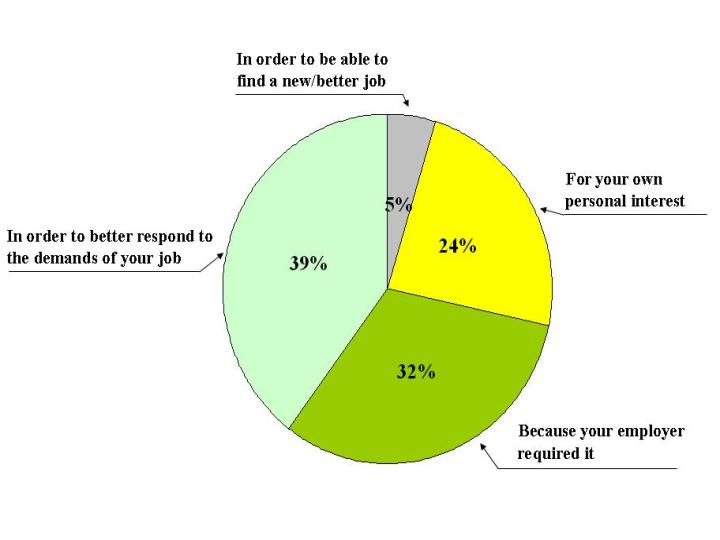
\includegraphics[width=7.5cm]{profKlausSchoemann-fig1.jpg}
    \caption{Reasons for taking part in training, EU 25 (Source: data from the Eurobarometer 2005, own calculations, Geerdes and Sch\"{o}mann 2006).}\label{fig1:profKlausSchoemann}
   \end{center}
\end{figure}

\newpage
\paragraph{Collaborations}
\begin{itemize}
\item Institute for Labour Studies (HIVA) \\ Catholic University Leuven \\ Dr. Tom Vandenberghe (co-ordinator)
\item Institute for Labour Studies (OSA) \\ University of Tilburg \\ Prof. Ruud Muffels 
\item Centre for Labour Market Policy Research (CAFO) \\ V\"axj\"o University \\ Prof. Dominique Anx\"o
\item Economic and Social Research Institute (ESRI), Dublin \\ Prof. Philip O'Connell 
\item Social Economic Research Rotterdam (SEOR) \\ University of Rotterdam \\ Prof. Jaap de Koning
\item Istituto per la Ricerca Sociale (IRS) Roma \\ Dr. Manuela Samek Hugo
\item Hugo Sinzheimer Institute (HSI) \\ University of Amsterdam \\ Prof. Ton Wilthagen; Dr. Els Sol
\item Institut f\"ur H\"ohere Studien (IHS), Wien \\ Prof Dr. Lorenz Lassnigg 
\item MATISSE, Centre National de la Recherche Scientifique, Paris I \\ Prof. Bernard Gazier
\item Institute for Employment Studies (IES) \\ University of Warwick \\ Prof. Ralf Rogowski 
\item McGill University, Canada \\ Prof. Axel van den Berg 
\item Universidad de Alcala, Madrid \\ Prof. Luis Toharia
\item Wissenschaftszentrum Berlin f\"ur Sozialforschung (WZB) \\ Prof. G\"unther Schmid 
\item Centre for Labour Market Research (CARMA) \\ Aalborg University \\ Prof. Per Madsen
\end{itemize}

\begin{bibunit}[apalike]
\nocite{*}
\putbib[profKlausSchoemann]
\end{bibunit}

\paragraph{Grants}

\begin{itemize}
\item European Foundation, 5th Framework Programme of the EU on ``managing social risks through transitional labour markets''. Co-financing by European Commission DG Employment as part of the mutual learning network. The research network consisted of 22 research groups in the European Union and a Canadian partner. The European Foundation in Dublin co-financed the data analysis of the Eurobarometer November 2005 data on labour mobility and geographical mobility in the EU. 
\item BMBF (PI: K. Sch\"omann): Qualification Needs in the OECD - Analysis and Implementation.
\end{itemize}

\subsection{Implications of the Aging Workforce for Learning and Work} 


\index{Sch\"omann, Klaus}

\paragraph{Research Team}
Klaus Sch\"omann (Professor), Anette Fasang (Doctoral Fellow), Paula Aleksandrowicz (Doctoral Fellow).

Germany faces a dual demographic challenge in the next 15 years. This consists in a considerable aging of the working-age population and of the total population, along with a shrinking size of the population of working-age. The size of the working-age population is projected to decline from 50 to 40 million people in 2020. Increasing the participation in employment of older workers is an important consequence of this demographic trend. To enable similar potentials of economic growth in the coming years not only more ``silver workers'' will have to work from each birth cohort, but the extension of the working live becomes likely scenario which is subject of our research interest in the field of productive aging. 

 Our second research theme deals with the links and exchangeability between human capital and social capital. We analyze the potential to increase voluntary work or civic engagement of older workers as the average life expectancy and fitness in older age increase. Thereby we assess the reversibility of retirement transitions and new combinations of market and non-market work in Western societies. 

 The part of sociology in the subproject "Learning" within the framework of the joint BMBF project concerns the area of learning participation and opinions of learning and their match with learning strategies and the learning culture of within a firm under the demographic aging of the employees and management. 

\begin{figure}[h]
  \begin{center}
    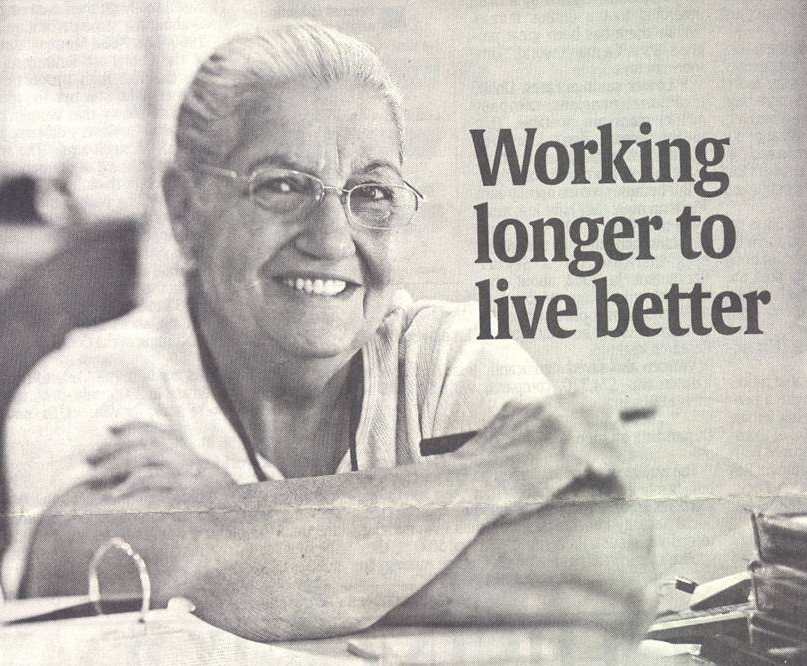
\includegraphics[width=7.5cm]{profKlausSchoemann-fig2.jpg}
    \caption{A challenging research agenda for life course sociology (Source: USA today 14.9.2006).}\label{fig2:profKlausSchoemann}
   \end{center}
\end{figure}

\textbf{Research Highlights 2006}

 Based on our first telephone survey of employees in part-time retirement in one firm we have produced a report on the results for the company executives. We have already achieved a faster turnaround from collecting survey data ourselves to data analysis and publication of results. The finding that even the retirement transition might be a transition, that can be reversed was received with some enthusiasm in the company as they are looking already for means to rehire some of their previous employees sent into early retirement. Similarly the combination of civic engagement of the enterprise and its former employees might constitute an interesting future potential of cooperation beyond the traditional employment relationship of dependent full-time employees in this firm. 

 Additionally we started to cooperate with the ``European initiative for the rights of future generations'' in the field of social policies. 


\paragraph{Collaborations}
\begin{itemize}
\item OECD Department of Employment and Social Affairs
\item Universit\'e Paris I, MATISSE \\ Maitre de Conf\'erences \\ Christine Erhel
\item University of V\"axj\"o  \\ Prof. Dominique Anx\"o 
\item OSA Institute for Labour Studies  \\ Dr. Frank Tros 
\item University of North Carolina at Chapel Hill  \\ Prof. Dr. Arne Kalleberg
\end{itemize}

\begin{bibunit}[apalike]
\nocite{*}
\putbib[profKlausSchoemann2]
\end{bibunit}


\paragraph{Grants}
\begin{itemize}
\item BMBF (PI: JCLL). K. Sch\"omann, C. Ro\ss nagel: subproject ``Learning / Training'' within the joint research project ``Effects of Matches/Mismatches between Aspects of Human and Social Capital, Corporate Strategy and Work Organization on the Physical and Mental Well-Being of Employees''. 
\item Consulting Project (PI: K. Sch\"omann, U. Staudinger): Retirement Processes in a Large Firm.
\item Consulting Project (PI: K. Sch\"omann): Evaluation of company-wide occupational health and safety trainings.
\item Executive Teaching for AutoUni in Wolfsburg by K. Sch\"omann.
\item DFG Travel Grant for Anette Fasang to present her first research results to the Sociology department at Yale, USA.
\item Grant by the European Sociological Association for Sara Geerdes for participation in a Summer School on Migration in Milano, Italy.
\end{itemize}

\subsection{Other Professional Activities}

\begin{itemize}
\item Consultant to OECD, European Commission DG Employment, Brussels and the European Foundation for the Improvement of Living and Working Conditions, Dublin.
\item Administrative Coordinator SISWO (Netherlands, 5th Framework Programme of the European Commission DG Research). 
\end{itemize}

\textit{Editorial Board Membership}

\begin{itemize}
\item Formation Emploi, Revue Fran\c caise de Sciences Sociales (since 2002).
\end{itemize}

 



\onecolumn
\newpage
\section{PhD Degrees}
\shorttitle{PhD Degrees}

\paragraph{2006} D\"orner, Jessica: ``A Self-Concept Measure of Personality Growth: Self-Concept Maturity (SCM). Development, Validation, and Age Effects''

Dissertation Committee: Prof. Dr. Ursula M. Staudinger (supervisor, IUB), Prof. Dr. Alexandra Freund (University of Zurich), Prof. Dr. Manfred Diehl (University of Florida, USA), Prof. Dr. Ulrich K\"uhnen (IUB), Prof. Dr. Britta Renner (IUB)

\paragraph{2006} Kessler, Eva-Marie: ``Intergenerational Relations as Facilitative Developmental Context'' 

Dissertation Committee: Prof. Dr. Ursula M. Staudinger (supervisor, IUB), Prof. Dr. Ute Kunzmann (IUB), Prof. Dr. Werner Greve (University of Hildesheim), Prof. Dr. Klaus Boehnke (IUB)

\paragraph{2005} Mickler, Charlotte: ``Self-related wisdom: Validation and age effects of a new measure of personal maturity'' 

Dissertation Committee: Prof. Dr. Ursula M. Staudinger (supervisor, IUB), Prof. Dr. Ute Kunzmann (IUB), Prof. Dr. Sigrun-Heide Filipp (University of Trier), Prof. Dr. Margrit Schreier (IUB)




\newpage
\section{Faculty} \shorttitle{Faculty}

\begin{tabular}{ll}
Dr. Godde, Benjamin	& Professor of Human Performance and Neuroscience\\
& \\
Dr. Kunzmann, Ute			& Professor of Psychology\\
& \\
Dr. Renner, Britta		&	Professor of Psychology\\
& \\
Dr. Rossnagel, Christian	&	Professor of Organizational Behavior (since 09/2006) \\
& \\
Dr. Sch\"omann, Klaus		&	Professor of Sociology\\
& \\
Dr. Schwender, Clemens	&	Professor of Communication Science\\
& \\
Dr. Staudinger, Ursula M.	&	Professor of Psychology\\
& \\
Dr. Voelpel, Sven			& Professor of Business Administration
\end{tabular}


\newpage
\section{Graduate Students and Postdoctoral Fellows}
\shorttitle{Graduate Students and Postdoctoral Fellows}

\begin{tabular}{lp{8cm}}
Aleksandrowicz, Paula	&	Graduate Student (Sociology)\\[0.8ex]

Babanin, Mikhail		&	Graduate Student (Human Performance)\\[0.8ex]

D\"orner, Jessica	& Graduate Student (Psychology; graduated 05/2006) and Postdoctoral Fellow (until 08/2006) \\[0.8ex]

Fasang, Anette		&	Graduate Student (Sociology)\\[0.8ex]

Fr\"uchtenicht, Jan-Dirk	&	Graduate Student (Business Administration since 09/2006)\\[0.8ex]

Geerdes, Sara-Izabella	&	Graduate Student (Sociology)\\[0.8ex]

Han, Zheng		&		Postdoctoral Fellow (Business Administration until 09/2006)\\[0.8ex]

Hartung, Freda-Marie			& Graduate Student (Psychology)\\[0.8ex]

Heidemeier, Heike		&	Postdoctoral Fellow (Psychology since 03/2006)\\[0.8ex]

Isichenko, Polina		&	Graduate Student (Business Administration)\\[0.8ex]

Kessler, Eva-Marie	& Postdoctoral Fellow (Psychology since 01/2006)\\[0.8ex]

Meyer, Jan			&	Graduate Student (Business Administration)\\[0.8ex]

Mocigemba, Dennis	&		Postdoctoral Fellow (Communication Science)\\[0.8ex]

M\"uhlig-Versen, Andrea	&	Graduate Student (Psychology)\\[0.8ex]

Noack, Martin		&		Graduate Student (Psychology since 03/2006)\\[0.8ex]

Oeberst, Andries	&		Graduate Student (Psychology)\\[0.8ex]

Otto, Siegmar		&		Graduate Student (Communication Science)\\[0.8ex]

Panzer, Martina	&		Graduate Student (Psychology)\\[0.8ex]

Richter, David	&			Graduate Student (Psychology)\\[0.8ex]

Siarov, Liuben	&			Research Associate (Sociology)\\[0.8ex]

Spivak, Youlia	&			Graduate Student (Psychology)\\[0.8ex]

Streb, Chris		&		Graduate Student (Business Administration)\\[0.8ex]

Tekie, Eden			&	Graduate Student (Business Administration)\\[0.8ex]

Voelcker-Rehage, Claudia	&	Postdoctoral Fellow (Human Performance)\\[0.8ex]

Zhao, Chunli		&		Graduate Student (Business Administration)
\end{tabular}

\newpage

\section{Visiting Scholars at the Jacobs Center}
\shorttitle{Visiting Scholars}

\textit{Dr. Pilvikki Absetz} (KTL Public Health Institute Helsinki, Finland)

 
\textit{Prof. Dr. Uschi Backes-Gellner} (Professor of Business Administration, University of Zurich, Switzerland): ``Demographical Change, Firm Demography and Productivity''


\textit{Dr. Lutz Bellmann} (Institut f\"ur Arbeitsmarkt- und Berufsforschung): ``Recruiting Elder Employees in Germany: Empirical Evidence from a Large-Scale Establishment Panel Survey''


\textit{Yael Benyamini, PhD} (School of Social Work, Tel-Aviv University)


\textit{Prof. Dr. Axel B\"orsch-Supan} (Professor of Macroeconomics and Public Policy, University of Mannheim, and Director, Mannheim Research Institute for the Economics of Aging - MEA): ``Macroeconomic Consequences of Demographic Change''


\textit{Dr. Hartmut Buck} (Fraunhofer Institut Arbeitswirtschaft und Organisation): ``Aging Workforce - Consequences for Enterprises''


\textit{Prof. Dr. Ekkehart Frieling} (Professor of Business Administration, University of Kassel): ``Work Conditions that Facilitate Learning''


\textit{Prof. Winifred A. Gebhardt, PhD} (Professor of Clinical and Health Psychology, Leiden University, NL)


\textit{Prof. Dr. Werner Greve} (Professor of Psychology, University of Hildesheim)


\textit{David Hevey, PhD} (School of Psychology, Trinity College Dublin)


\textit{Dr. Dagmar Hoffmann} (Academy of Film and Television, Potsdam-Babelsberg): ``Older People, Media Activities and Movie Preferences - What Does Research Tell Us?''


\textit{Prof. Arthur Kramer, PhD} (Professor of Human Performance, University of Illinois, USA, and Director of the Biomedical Imaging Center at the University of Illinois): ``Fitness Effects on Brain and Cognition''


\textit{Prof. Dr. Marius Leibold} (Professor of Strategic International Management, University of Stellenbosch, South Africa)


\textit{Prof. Dr. Susan Michie} (Professor of Health Psychology, University College London)


\textit{Prof. Dr. Ekkehart Nuissl von Rein} (Professor of Educational Science, and Scientific Director of the German Institute for Adult Education - DIE): ``Development of European Perspectives of Adult Education''


\textit{Prof. Dr. Christel Salewski} (Hochschule Magdeburg-Stendal, FH)


\textit{Dr. Caroline Schuster-Cordone} (University of Bern, Switzerland)


\textit{Prof. Dr. Norbert Schwarz} (Professor of Psychology, University of Michigan, USA): ``Would you be happier if you were younger and richer?''


\textit{Prof. Dr. Ralf Schwarzer} (Professor of Psychology, Free University of Berlin): ``How to Conceptualize Health Behavior Change: Stage Models vs. Continuum Models''


\textit{Dr. Vegard Skirbekk} (International Institute for Applied Systems Analysis, Austria): ``Productivity Potential over the Life Cycle. The Changing Importance of Age-Specific Abilities'' 


\textit{Dr. Vera Soares} (Department of Psychology, University of the Minho, Portugal)


\textit{Prof. Dr. Thomas Staufenbiehl} (Professor of Psychology, University of Osnabr\"uck)


\textit{Prof. Dr. Clemens Tesch-R\"omer} (Professor of Psychology, Free University of Berlin and Director of the German Centre of Gerontology - DZA, Berlin): ``Health in an Aging Workforce - Results from the German Aging Survey''


\textit{Irina Todorova, PhD} (Bulgarian Academy of Sciences)


\textit{Prof. Dr. Gert Wagner} (Professor of Economics, Berlin Technical University, and SOEP Research Director, Deutsches Institut f\"ur Wirtschaftsforschung): ``The German Socio-Economic Panel Study (SOEP) as a Basis for Life Course Research''


\textit{Prof. Dr. Klaus Willimczik} (Professor of Human Performance, University of Bielefeld): ``The Effectiveness of Teaching and Learning Sport Motor Skills Across the Lifespan - Theoretical and Meta-Theoretical Aspects''


\end{document}
